% Template author: Johannes Demel
% Document class provides standardized title page + needed extras.
\documentclass{cel-thesis/cel-thesis}
\thesisTitle{TBS}
\thesisType{Master's Thesis}
\thesisAuthor{Nicolas Cuervo-Benavides}
\thesisAdvisor{Dr.-Ing. Holger Jäkel}
\thesisHeadOfInstitute{}
%\thesisHeadOfInstitute{Dr.-Ing. Holger Jäkel}
\thesisSupervisor{MSc. Felix Wunsch}
\thesisStartDate{17th May 2017}
\thesisEndDate{6th December 2017}
\thesisSignatureDate{06.12.2017}
\thesisLanguage{english} % english or ngerman
\thesisCC{FALSE}
\thesisPythonWatermark{FALSE}


%%% LANGUAGE SETTINGS %%%%%%%%%%%%%%%%%%%%%%%%%%%%%%%%%%%%%%%%%%%%%%%%%%%%%
% additional Hyphenation rules
\hyphenation{non-para-metric repro-gra-mmable}
% Settings for bibliography
\usepackage{babelbib}
\setlanguage % set correct language as selected above

%%% PACKAGES %%%%%%%%%%%%%%%%%%%%%%%%%%%%%%%%%%%%%%%%%%%%%%%%%%%%%%%%%%%%%%%%%
% Add all the packages you feel like you need them.
% You'll need it.
% automatically expand/abbreviate terms.
\usepackage{caption}
\usepackage{subcaption}
\usepackage{todonotes} % great for draft annotations

% Added additionally to the template
\usepackage{standalone} % To add tikz figure as standalone elements
\usepackage{tikz}  % To add tikz figures
\usepackage{array} % To use alignment such as m{} or b{} in tables
\usetikzlibrary{datavisualization}
\usetikzlibrary{positioning}
\usetikzlibrary{arrows,calc,fit}
\tikzset{line/.style={draw, thick, -latex'}}


%%% DEFINITIONS %%%%%%%%%%%%%%%%%%%%%%%%%%%%%%%%%%%%%%%%%%%%%%%%%%%%%%%%%%%%%%%%%
%% pretty C++ print.
\def\CC{{C\nolinebreak[4]\hspace{-.05em}\raisebox{.4ex}{\tiny\textbf{++}}}}

\begin{document}
\pagenumbering{roman}  % all the preliminaries should be counted roman style
\maketitle
%% preliminaries
  \chapter*{Abstract}

This thesis evaluates different machine learning techniques for effective spectrum awareness on \ac{CR} interweave systems. In the last decades, access to the electromagnetic spectrum has been granted to the highest bidder on \emph{spectrum auctions}. The auction winner is thereafter entitled to use a definite portion of the spectrum in a way which fits the best to the technology or service that he wants to provide. But, with increasing demand for this natural resource, it is imperative to find techniques that allow a more effective use of the spectrum, such as spectrum sharing.\\

Spectrum sharing has been an ongoing topic of research in the last few years for the purpose of being part of the 5G communications systems, as well as for generally mitigating spectrum scarcity. The \ac{CEL} has actively worked on this issue with the use of \ac{SDR} and \ac{CR} devices. \ac{CR} devices have, conceptually, a \emph{learning stage} where they observe signals from the outer world in order to learn how to react accordingly, which consequently serves as a catalyst for the introduction of \ac{ML} to accomplish this purpose. Recently, \ac{CEL} has very successfully taken part in the \ac{DySpan} spectrum challenge competitions which deal specifically with this matter. In these competitions, a communication system with higher priority, also known as a \ac{PU}, is set to make use of a certain central frequency and \ac{BW} (divided into four channels) sending packets in a bursty fashion, randomizing the way it accesses the spectrum over ten different scenarios that vary its channel ocupation, frequency hopping pattern, packet length and inter-packet delay. The objective of these competitions is to implement a communication system with lesser priority, also known as a \ac{SU}, that identifies effectively the scenario that the \ac{PU} is using, and takes advantage of this information to access the spectrum in a way that interferes the least with the ongoing communication. This thesis uses the DySpan Spectrum Challenge 2017 setup as testbed and focuses on evaluating techniques used to identify the way the \ac{PU} is accessing the spectrum by the means of \ac{ML} and \ac{DL}.\\

Within the implementation of the challenge's testbed the specific scenario that the \ac{PU} uses for its transmission can be controlled, and this ability is used to record labeled samples over the specified bandwidth during a certain amount of time in order to generate a composite dataset, from which the scenarios that it uses are learned thenceforth using supervised learning. Additionally, the transmission power of the \ac{PU} is also varied in order to generate samples with different \ac{SNR}, to ensure that the \ac{ML} models learn how to classify under a diversity of signal power conditions. The learning methods are separated into two categories, based on the type of preprocessing that input data undergoes:

\paragraph*{Feature-based learning:} specific information is extracted from the recorded data as so-called \emph{features}, and then is used as an input into \ac{ML} algorithms. Then a benchmark between the K-nearest neighbors, decision trees, and \ac{SVM} is presented demostrating how well these algorithms are able to classify the correct scenario based on the extracted features. This method relies on a energy detection scheme to generate the features, which presents a limitation when the \ac{PU} is transmitting with low SNR.
\paragraph*{Spectrogram-based learning:} data preprocessing here consist of generating spectrograms that are fed into convolutional neural networks for them to be classified using image recognition techniques. Different optimizers, such as the stochastic gradient descent, adamax, and adadelta, are used to achieve an understanding of their convergence speed as well as their accuracy. This method is independent of the \ac{PU} SNR, as the spectrograms are generated directly from the input data regardless of its spectral content.\\

The performance of these methods is analyzed with respect to their accuracy on classification over the test dataset, along with the time they take to classify a data sample. These parameters serve as figures of merit to determine how viable it is to use these algorithms in real-time applications. Lastly, a demonstration of the performance of the regarded classification models is presented using GNU Radio, where the \ac{PU} scenarios are classified in real-time. This work shows that with a relatively little amount of data confident spectrum awareness can be achieved using learning techniques, without the need of pinning down a specific analytical description of the way the spectrum is being utilized by other actors in a communication system.\\

This thesis culminates in a conclusion on the feasibility of using the analyzed \ac{ML} algorithms in real-time scenarios. Based on the results achieved, it can be confidently affirmed that decision trees provide the best trade off between accuracy and prediction time for this specific use case for feature-based classification. On the counterpart, \ac{SVM} do not provide satisfactory results, having a about 10\% less accuracy than the other two analyzed models while taking about 2500 times longer to provide a prediction than decision tree classifiers, and about 50 times longer than K-nearest neighbors classifier prediction, making them unsuitable for this application. Furthermore, it is found that image classification using a convolutional neural network with the adadelta optimizer provides a reliable classifier with as little as 300 iterations of training, which makes the spectrogram-based learning appealing over the feature-based learning as it does not depend on the \ac{PU} signal power to provide a prediction.
		% a MUST, few pages abstract

%% main document
\cleardoublepage
\pagenumbering{arabic} % now old school arabic enumerated pages.
  \tableofcontents 		% a MUST
  \cleardoublepage		% make sure multipage TOCs are numbered correctly.
  \acresetall
\chapter{Introduction}\label{ch:intro}

Back in 1999, Joseph Mitola III coined the term \ac{CR}\cite{Mitola1999} as a way to enhance the \ac{SDR} capabilities by the means of a dynamic model that, based on human intervention, improved the flexibility of devices by making them fully configurable and capable of adapting to the communication system's needs, suitable to react to the changes it the surrounding environment. A formal definition for the \ac{CR} concept provided at \cite{Haykin2005} encloses the term nicely by describing it as a wireless system that is \emph{intelligent and aware of its surroundings}, whilst being able to learn, adapt and react to changes in the environment, by modifying its operation parameters such as the transmission power, the modulation scheme and its carrier frequency in real-time. Analogously, Jondral \cite{Jondral2005} adopts the short definition for \ac{CR} as "an \ac{SDR} that additionally senses its environment, tracks changes, and possibly reacts upon its findings", becoming an autonomous unit with the potential of using the spectrum efficiently.\\

\ac{CR} systems are intended to be immerse in a network, where it interacts with other systems that could be cognitive or non-cognitive radios. According to \cite{Goldsmith}, \ac{CR} is grouped under three paradigms: underlay, overlay and interweave. The \emph{Underlay Paradigm} allows the \ac{CR} system to operate under acceptable levels of interference, determined by an interference threshold. Here, the \ac{CR} is commonly called a \ac{SU}, providing priority to the other systems in the network which it should not significantly interfere, known also as \ac{PU}. In the \emph{Overlay Paradigm}, the cognitive transmitter knows information about the other transmitters in the network, such as their codebooks and modulation schemes. In addition, this model assumes that message that is being transmitted is known by the \ac{CR} when transmission by a non-cognitive system is initiated. This provides the cognitive system with multiple choices on how to use this information: for instance, it can be used to mitigate or completely cancel a possible interference happening in the network during transmission. Additionally, the cognitive system could also retransmit this message to other non-cognitive systems in the network, acting as a relay and, effectively, assist increasing the \ac{SNR} of the non-cognitive system to a level equivalent to the possible decrease due to \ac{CR} transmissions. The \emph{Interweave Paradigm}, or opportunistic communication, identifies temporary space-time-frequency gaps where it can intelligently allocate its transmission, increasing the available resource utilization and minimizing the interference with other active users. Hybrid schemes are also actively being developed \cite{Wu2007} \cite{Kaushik2015} \cite{Wunsch2017a}, where characteristics from different paradigms are combined in order to achieve an effective use of the available communication resources.\\

The main characteristic required to apply any of the aforementioned paradigms is awareness, being it in regard of location, spectrum, time, etc. Awareness is achieved by the means of \emph{the cognition cycle} \cite{Mitola1999}, which can be seen in Fig.~\ref{fig:cognition_cycle}, which enfolds the way the \ac{CR} parses the stimuli from the outside world in order to plan accordingly the proper reactions. This cognition cycle revolves around the following concepts

\begin{figure}[htb]
    \centering
      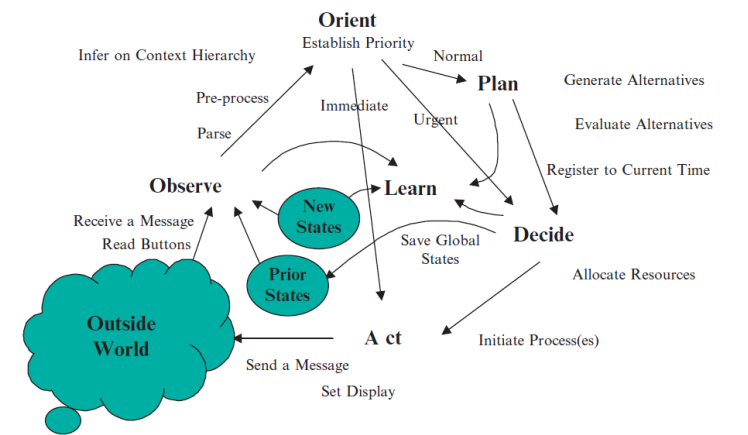
\includegraphics[width=0.8\textwidth]{figures/cognition_cycle.png}
      \caption{The cognition Cycle\cite{Mitola1999}}
      \label{fig:cognition_cycle}
\end{figure}

\begin{itemize}
    \item Observation: the \ac{CR} receives any signals from the external world, which can contain any type of information that the system can use in its favor and the favor of a better use of its resources.
    \item Orientation: The \ac{CR} determines the priority from the received signal as well as the type of reaction based on it.
    \item Planning: results from a normal-level priority, where a plan is generated and the sequence of actions to be taken are established.
    \item Decision: selects among the plan candidates the best proposal and allocates the necessary resources for its carrying-out.
    \item Acting: initiates the decided processes.
    \item learning: is an integration of observations and decisions, based on past and current states that are compared with expectations. When an expectation is met, the system achieves effectiveness. When not, observations are recorded and kept for further learning.
\end{itemize}

These aspects of \ac{CR} come in handy when trying to solve one of the current major issues of communication systems: Spectrum Scarcity. The access to radio spectrum is highly regulated by government agencies such as the \ac{Ofcom}, the \ac{FCC} and the \ac{ITU}, and its access has been historically granted to the highest bidder on so-called \emph{Spectrum Auctions} \cite{Jondral2005} \cite{Staple2004}. Therefore, the seek of new technologies that allow a more efficient access to the spectrum is paramount. In an effort to find effective solutions for this increasing issue, the \ac{IEEE} created a Standards Committee back in 2005 which, in association with the \ac{ComSoc} and the \ac{EMC} dealt with the generation of standards for dynamic spectrum management. This committee was dissolved between 2007 and 2010 and, after organizational restructuring, the functions of standardization and spectrum management was handed to the \ac{SCC} - \ac{DySpan} \cite{IEEEDySPAN2015}. As part of this efforts to motivate state-of-art research in this regards, \ac{DySpan} has organized since 2007 the \emph{IEEE International Symposium on Dynamic Spectrum Access Networks} \cite{Comsoc}. Additionally, \ac{DySpan} has embolden the healthy competition since 2015 by introducing the \emph{Spectrum Challenge}, consisting on inviting team worldwide to solve a problem related with dynamic access to the spectrum and 5G implementations. The participating teams are given a set of requirements and limitations, but are encouraged to push this limits with creativity and innovation. The \ac{KIT}, represented by the \ac{CEL}, has taken part in these competitions achieving outstanding results, being awarded with the \emph{Subjective Winner} award on 2015 \cite{Kaushik2015} and the \emph{Best Overall Solution} on 2017 \cite{Wunsch2017a}. This thesis utilizes the setup used at the 2017 spectrum challenge as base testbed. Fig.~\ref{fig:dyspan_setup} shows the main characteristics of this setup.

\begin{figure}[htb]
    \centering
      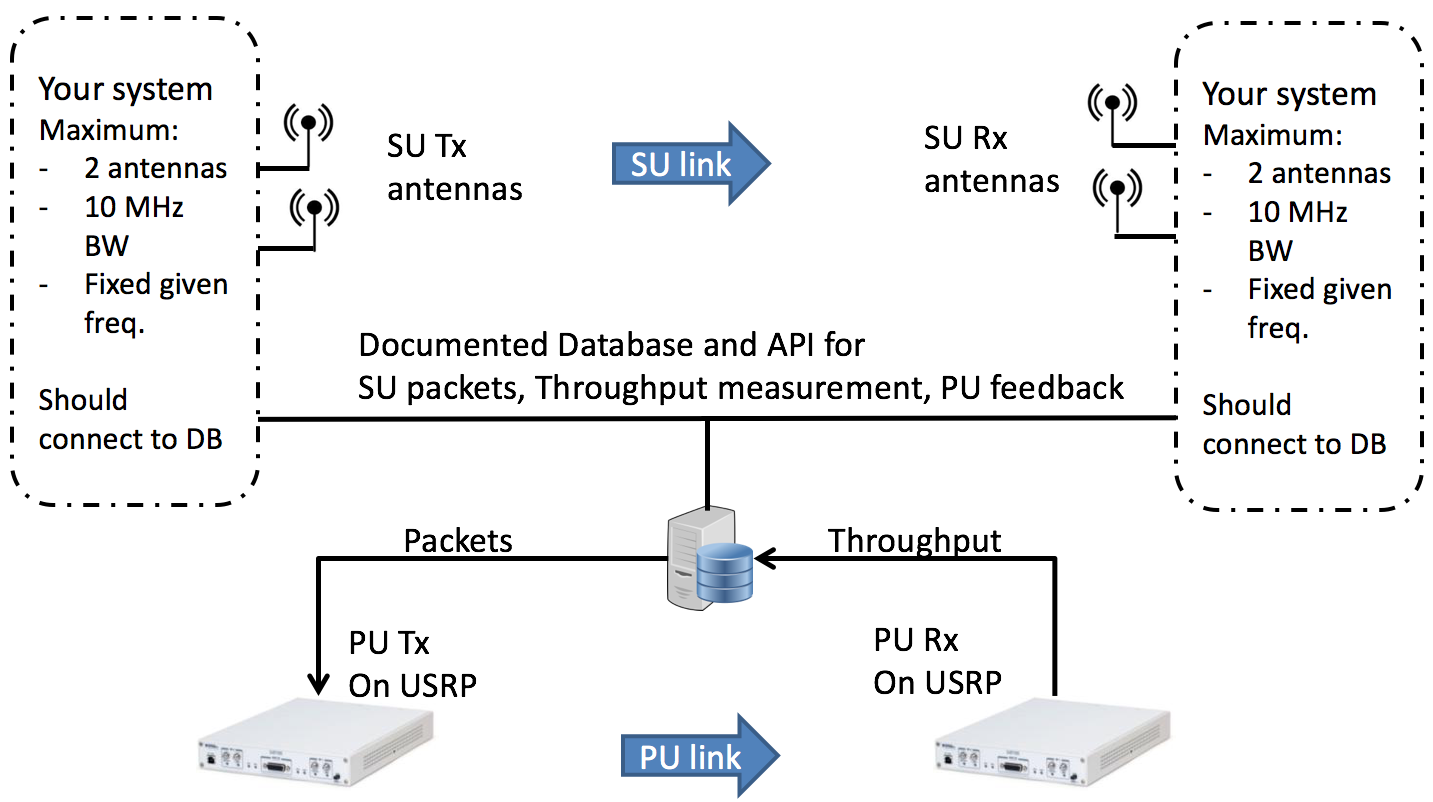
\includegraphics[width=0.8\textwidth]{figures/dyspan_set.png}
      \caption{The DySpan Spectrum Challenge Setup \cite{Dyspanchalle}}
      \label{fig:dyspan_setup}
\end{figure}

By using this configuration and keeping the hardware and overall physical considerations (such as \ac{BW}, number of antennas and central frequency),
the idea of the challenge was to achieve the maximum throughput between the proposed \ac{SU} systems, while interfering as little as possible with the existing \ac{PU}. The competition consisted of two phases: during phase one the situational awareness of the proposed \ac{CR} system is put under test, as it need to correctly identify the set of \ac{PU} transmission parameters:

\begin{itemize}
    \item Bandwidth and Carrier Frequency: along the 10MHz of maximum \ac{BW} divided in four subchannels of 2.5MHz each, it needs to be detected if the \ac{PU} is using one, two or four channels for its transmission. Effectively, it is needed to determine which frequencies are being used (identify the frequency hopping pattern) and when are they being used.
    \item Packed length: the \ac{PU} transmitter sends packets in a bursty fashion to the corresponding receiver using packets of 100 or 1000 bytes.
    \item Inter arrival time between packets: the time between a packet transmission might vary from a situation to another. This times could be deterministic for some scenarios, as well as stochastic for others following a Poisson distribution. Correctly identifying the length of the packet, as well as the inter packet time of the current situation, allows to effective opportunistic access to the spectrum.
\end{itemize}

With this characteristics, a set of 10 different scenarios is built, whose parameters are depicted in Table~\ref{table:scenarios}

\begin{table}[h!]
    \centering
    \begin{tabular}{| >{\centering}m{5em}| m{12cm} |}
        \hline
        \textbf{Scenario} & \multicolumn{1}{|c|}{\textbf{Description}} \\
        \hline\hline
        0 & Single random channel, deterministic interpacket delay of 5ms \\\hline
        1 & Single random channel, deterministic interpacket delay of 10ms\\\hline
        2 & Two random channel hopping, deterministic interpacket delay of 5 ms\\\hline
        3 & Four random channel hopping, deterministic interpacket delay of 10 ms\\\hline
        4 & Two random channel hopping, deterministic interpacket delay of 5ms\\\hline
        5 & Four synchronous channels, deterministic interpacket delay of 5ms\\\hline
        6 & Four synchronous channels back-to-back, deterministic interpacket delay  of 2ms\\\hline
        7 & Four asynchronous random channels, Poisson distributed interpacket delay with mean of 20ms\\\hline
        8 & Four asynchronous random channels, Poisson distributed interpacket delay with mean of 10ms\\\hline
        9 & Four asynchronous random channels, Poisson distributed interpacket delay with mean of 5ms\\
        \hline
    \end{tabular}
    \caption{Scenario description}
    \label{table:scenarios}
\end{table}

The second phase of the competition regards the benchmark of the performance of the proposed \ac{SU} implementation, where aspects such as innovation of the used waveform, machine learning algorithms used, and opportunistic access to the spectrum were considered. The proposed solutions, including the one proposed by \ac{CEL}, can be found at \cite{Wunsch2017a}, \cite{Papadakis2017},  \cite{Paisana2017} and \cite{Lackpour2017}, where a high level of innovation and state-of-the-art research is compiled.

Being clear that \emph{awareness} has been a primordial characteristic of \ac{CR} since the conception of the concept until now, understanding that this is an area that invites to further research and considering the uprising research in the field of \ac{AI} algorithms, this work focuses on the learning aspect of \ac{CR}, using the setup from Fig.~\ref{fig:dyspan_setup} in order to effectively identify the scenarios described at Table~\ref{table:scenarios}. Previous research on this field covers aspects such as modulation recognition \cite{Oshea2016}\cite{Oshea2016d}, resource allocation \cite{Zappone2016}, autoencoding and optimization of MIMO systems \cite{Oshea2017}, dynamic spectrum management \cite{Haykin2005} and context awareness \cite{Paisana2017}\cite{Wunsch2017}.


The outline of this thesis is as follows:  an introduction to \ac{AI}, focused on \ac{ML} and \ac{DL}, alongside the most used algorithms used in academic and industrial fields is presented in chapter~\ref{ch:ml_intro}. General techniques to avoid phenomena such as underfitting and overfitting of the \ac{ML} are, as well, portrayed. Chapter~\ref{ch:implementation} describes the details of the testbed set up, the measurement of the data and the implementation of the machine learning models. The evaluation of the learning models is then presented in ~\ref{ch:evaluation} with metrics of performance. The models are put into a live implementation, where the performance of the algorithms is put into test by classifying the scenarios of Table ~\ref{table:scenarios} in real-time - This is presented in chapter~\ref{ch:live}. Lastly, the conclusions and future work are summarized in chapter~\ref{ch:conclusions}.
		% include chapter introduction.tex
  \acresetall
\chapter{Artificial Intelligence}\label{ch:ml_intro}

\section{Overview}
\emph{Intelligence} as a concept has been a topic of exhausting research in fields such as neurology, philosophy, neuroscience, neurobiology, datascience, among others. The Oxford dictionary defines intelligence as \emph{"the ability to acquire and apply knowledge and skills"} \cite{Oxforda}. The first part of this definition applies to what is known as "learning", which is according to the accepted definition of the term as well \cite{Oxford}, and that supports, from the etymology, the importance of the process of learning on intelligence.\\

Jeff Hawkins, a dedicated neuroscientist and author, has approached the subject from the engineering and medical flanks, analysing the structure of the brain and having the perspective of the possibilities of replicating artificially the most sophisticated type of intelligence found on Earth: the human. In his book \emph{On Intelligence} \cite{HawkinsJeff2004}, he captures his findings after inspecting the brain cortex and making a parallel between humans and machines. According to Jeff, \emph{"it is the ability to make predictions about the future that is the crux of intelligence"}, and these predictions are based on the experiences from which the intelligent being has learnt, making decisions that lead it to the best possible known result. In order to create artificially a so-called \emph{intelligent agent}, scientist have put extensive effort first on trying to replicate the known intelligence \cite{Brooks1991}\cite{Reed2007}\cite{Hawkins}, taking the approach of generating a machine that is human-like and that behaves like one, being able to observe its surroundings, learn from stimulus that come from the real world, adapt to changes in those surroundings, plan accordingly to foreseeable process (therefore, make predictions), make decisions and act appropriately. These are the characteristics that Mitola \cite{Mitola1999} described in the cognition cycle for \ac{CR}, which can be applied to any intelligent agent and, consequently, motivate the further research of \ac{AI}.\\

\ac{AI}, however, encircles a variety of disciplines that are in themselves a complete course of research, as it can be seen in Fig~\ref{fig:ai}. This work focuses only in the top branch: machine learning. However, given the slight differences regarding implementation, a separate section will be dedicated solely to deep learning.

\begin{figure}[htb]
    \centering
      \includestandalone[width=\textwidth]{figures/ai_tree}
      \caption{Artificial Intelligence}
      \label{fig:ai}
\end{figure}

\section{Machine Learning}
\ac{ML} encloses the process of taking a data set that represents any phenomena and learning from it. Any type of being that is capable of learning from previous experiences is showing a kind of intelligence, as it interiorizes the stimulus/data and reacts accordingly when it presents itself again. The vast majority of living beings have this capacity, being the humans who have the lead on its effectiveness. Identifying objects, speaking languages, and reacting to any sensorial stimulus is a result of a successful learning process. \\

Generally speaking, learning from data is done when no there is no analytic solution to an encountered situation, but there is enough data to adapt to the it, generating an empirical solution to a problem that cannot be mathematically a-priori described, but that follows a specific pattern\cite{Yaser}. Just as humans do, the idea of machine learning is to generate intelligent agents computationally - teach computers to learn. The idea is as follows: a machine learning algorithm is given a set of data from which it can extract specific information that tells it the specifics about the data. With enough information, the computer is able to make predictions about other data in a different point of time if this data presents the same characteristics.

Although there is no specific mathematic representation of the specific problem to solve, many \ac{ML} algorithms relay heavily on mathematic definitions and optimization theory. Further information regarding \ac{ML} algorithms can be found in section~\ref{ch:ml_algs}. Yet is this versatility provided by the fact of not needing to pin down the specific analytic description of the problem which has impulsed this methodology into several fields of knowledge, being nowadays applied to solve problems such as financial forecasting\cite{Bose2001}, medical diagnosis\cite{Kononenko2001}, entertainment\cite{Bennett2007} and communications systems (such as this thesis), among others. Examples of everyday problems that are suitable for \ac{ML} implementation are:

\begin{itemize}
    \item Ranking links and clicks for a better web search engine and advertisements.
    \item Custom user recommendations based on purchases/rents/views.
    \item Prediction of markets and stock exchange.
    \item Dating sites with reevaluation of algorithms based on successful matches.
    \item Financial fraud detection.
    \item Supply chain optimization
    \item Biotechnology research acceleration by sequencing and screening of DNA and protein/compound structures.
    \item National security based on enormous surveillance data.
\end{itemize}

There are three types of learning: supervised-, unsupervised-, and reinforcement learning. Each of them  has specific characteristics, which are explained in the following subsections.
\subsection{Supervised Learning}
Is the type of learning where, in addition to the input dataset, the desired outputs for those given inputs are given to the \ac{ML} algorithm for training. There are two types of supervised learning:
\begin{itemize}
    \item \textbf{Classification:} its main goal is to predict a \emph{class label} from a determined set of choices. If the number of choices is two, the model corresponds to a \emph{binary classification}. As it has only two options, it is suitable for problems whose expected answer is of the form "yes/no", "present/not present", "valid/invalid". For a greater number of classes the model corresponds to a \emph{multiclass classification}. Examples of classification are:
        \begin{itemize}
            \item Determining whether an email is spam or not constitutes a binary classification problem.
            \item Identifying the zipcode from handwritten digits on an envelope is a multiclass classification problem.
            \item Determine whether a tumor is benign based on size and shape data constitutes a binary classification problem
        \end{itemize}
    \item \textbf{Regression:} its purpose is to predict a continuous behaviour, such as a trend, or a floating-number, and it is this continuity what sets it apart from the classification models. Examples of regression are:
        \begin{itemize}
            \item Predict the value of the stock market
            \item Determine the expected amount of crops yield from a plantation based on data such as previous yields, weather history, etc.
        \end{itemize}
\end{itemize}

\begin{figure}[htb]
    \centering
      \includestandalone[width=\textwidth]{figures/knn_accs}
      \caption{Artificial Intelligence}
      \label{fig:knn_accs}
\end{figure}


\subsection{Unsupervised Learning}
\subsection{Reinforcement Learning}

\subsection{Training Models}
\subsection{Testing Models}
\subsection{Model Evaluation}
\subsubsection{Overfitting}
\subsubsection{Underfitting}
\subsection{Feature Engineering}
\subsection{Machine Learning algorithms}\label{ch:ml_algs}
\subsubsection{K-nearest Neighbors}
\subsubsection{Support Vector Machines}
\subsubsection{Binary trees}

\section{Deep Learning}
\subsection{Neural Networks}
\subsection{Convolutional Neural Networks}
\subsection{Optimization of Cost Functions}


  \acresetall
\chapter{Testbed Implementation}\label{chapter:implementation}\label{ch:implementation}
This chapter depicts the tools and procedures used in the set up and data preparation prior the machine learning procedures. It includes the steps taken since the start of the work until the moment the first \ac{ML} algorithm started to train. First, an overview of the software and hardware tools is given. Afterwards, a short explanation on the available \ac{ML} libraries and frameworks is presented, along with the reasoning behind their choosing for this work. Lastly, process of measuring the data and preprocessing it is explained in detail, for the data to be ready to be applied to the learning models.
\section{Software Defined Radio approach}
As stated in the introduction of this thesis, \ac{SDR} and \ac{CR} play an important role in modern communication systems, and is the framework used for most projects at the \ac{CEL}, not only being used as a tool but also being actively contributed to with research results, but also acting as an active agent on open-source improvements. The software and hardware frameworks used are the following:
\subsection{GNURadio}
\begin{figure}[htb]
    \centering
      
\includegraphics[width=\textwidth]{figures/gnuradio_logo}
      \caption{GNURadio logo}
      \label{fig:gnuradio}
\end{figure}
GNURadio \cite{GNURadio2016} is a free and open-source toolkit that provides a large library of signal processing blocks that can be used for several software-defined radio applications. Its functionality does not require a device in the loop, which allows the users to simulate complete communications systems only on a computer. This includes signal sources, modulators and demodulators (such as \ac{PSK} and even \ac{OFDM}), dynamic channel simulators (and virtually any digital filter implementation), math operators, and a plethora of other digital signal processing implementations that have served purposes in academy, research, amateur radio hobbyist and even some government entities. Additionally, thanks to the support for several defined radio hardware \cite{gnuradiohw}, GNURadio grants the capability of transmitting (given the user has a rightful license for this purpose) and receive real signals and process them thoroughly.\\

The usual usage of this software is as follows: the user has a problem or an idea that requires digital signal processing, such as decoding a radio signal or implementing a novel communications' protocol. As said, GNURadio includes several algorithms that serve this purpose, and they are enclosed in so-called blocks. These blocks can then be connected to one another, generating a flow that the signal follows, in a so-called flowgraph, where each block takes a determinate amount of inputs, each input also taking a determinate amount of samples, that undergo the signal processing that the block entitles, and then the block presents its outputs to the next block downstream. If the library provided by GNURadio does not contain implementations that suffice the user needs, new implementations are easily added by the means of a so-called \emph{\ac{OOT}} module, where the user can provide additional applications, and characteristic that makes the scalability of GNURadio a transparent procedure. Lastly, if the user believes that custom implementation can serve a common purpose and other users, the \ac{OOT} can be made public following the open source standards, and this way other users can benefit from the same implementation and probably even contribute to it. An extensive collection of \ac{OOT} that have followed this open source mentality can be found at \ac{CGRAN} \cite{CGRAN}.\\

Regardless of the amount of inputs and outputs on a block, the amount of items required for the algorithm within determines the type of the block:

\begin{itemize}
    \item If for each output produced the block requires only one input item (1:1), then it is a \emph{sync} block.
    \item If the block requires N input items in order to generate 1 output item (N:1), the block is a \emph{decimation} block.
    \item If the block generates M output items for each 1 input item (1:M), the block is a \emph{interpolation} block.
    \item If the block requires to be extended flexibility, requiring N input items for each M output items produced (N:M), the block is a \emph{general} block.
\end{itemize}

Most of the blocks are written in a parametrizable fashion, serving multiple purposes with the same implementation by allowing the user to set different settings which can go from the general point of view, such as the vector length of the signal and its data type, to very specific and detailed parameters such as the taps of a filter or the description of a preamble. \\

The library of algorithms is organized in modules that have a common purpose, and within these modules you find blocks that help achieve that purpose. Examples of such modules are the “gr-qt” module contains the blocks that are intended to be used for visualization purposes using Qt \cite{Qt} and, within this module, blocks such as a “Time sink” and a “Frequency Sink” are found, which are written using Qt and serve as a scope and as a spectrum analyzer, respectively. Another example, more specific, is the gr-channels module, where the user can find different implementations for parametrizable channel simulators, such as fading, frequency selective, and dynamic channel models, among others. Most of these blocks are written in C++ and python, where each block is, in end effect, a class. In the same programming jargon, the module is a namespace. Therefore, the end user is expected to feel comfortable understanding (and, optimally, using-/writing-) these programming languages in order to be able to use these blocks to the fullest. The interconnection of the blocks, i.e. the flowgraph, is written using Python. For the C++ blocks to be available in the Python interface of the flowgraph, this C++ implementation is translated into Python domain by making use of the \emph{\ac{SWIG}}. In addition, multiple blocks can be grouped into a single block that serves a specific purpose, and this is called a hierarchical block.\\

Although coding to the base of the modules and blocks gives the user total control of the details, it is not the only way of getting things done while using GNURadio. The software comes with a \ac{GUI} called \ac{GRC}, which allows the user to drag-and-drop blocks into a canvas and connect them directly with the ease of a click. Even experienced users grab a hold on this \ac{GUI} as it provides ease and versatility along with a visible flowgraph that is easy to understand not only for the user but also to other users whose interest has been drawn to a specific application.\\

In order to use GNURadio, the recommended installation is done by the means of \ac{PyBOMBS} \cite{PyBOMBS}, which also allows installation of the modules listed at \ac{CGRAN}.

\subsection{Universal Software Radio Peripheral}
\begin{figure}[htb]
    \centering
      
\includegraphics[width=0.5\textwidth]{figures/ettus_logo}
      \caption{Ettus Research's logo}
      \label{fig:ettus}
\end{figure}

One of the \ac{SDR} devices that is supported by GNURadio is the \ac{USRP}, which is developed and produced by the company \emph{Ettus Research\texttrademark} \cite{Ettus}. This company has been a one of the most representative suppliers of \ac{SDR} devices around the globe, and these devices are reknown by its outstanding performance and versatility.\\

During the complete \ac{DySpan} spectrum challenge competition, three different \ac{USRP} devices where used for both \ac{PU} and \ac{SU}. The \ac{PU} used for the transmitter and the receiver the \ac{USRP} X310, which can be seen at Fig.~\ref{fig:x310} \cite{X300}. This device counts with two wide-\ac{BW} \ac{RF} daughterboard slots and a large customizable Xilinx Kintex-7 FPGA. Additionally, it has the capability of using high-speed interfaces such as 10gigE and PCIe, with which a maximmum of 200MS/s full duplex can be travel through the transport link. This \ac{USRP} covers from 10MHz until 6GHz, but based on the daughterboard selected, which serves as \ac{RF} frontend, the frequency of operation of the device can vary.\\

As for the \ac{SU} that was presented by the \ac{KIT} \ac{CEL} group, the transmitter used an \ac{USRP} N210, depicted in Fig~\ref{fig:n210} \cite{N210}. The N210 has a Xilinx Spartan 3A-DSP 3400 FPGA, and can hold up to 100MS/s through a 1gigE link that connects it to a host machine.  This device also requires an \ac{RF} daughterboard as frontend, for which in the \ac{SU} implementation the UBX-40, shown in Fig~\ref{fig:UBX} \cite{UBX}, was used. This daughterboard can operate from 10MHz to 6GHz, providing an instantaneous \ac{BW} of 40MHz. As for the receiver, a B210, shown in Fig~\ref{fig:b210} \cite{B210}, was used. This \ac{USRP} is a fully integrated, two channel device that operates from 70MHz to 6GHz without the need of additional \ac{RF} frontend configuration. It provides Full duplex, MIMO (2 Tx - 2Rx) operation up to 56 MHz of instantaneous \ac{BW}. Furthermore, it counts with a convenient USB 3.0 connection that also serves as power feed.\\

Although this devices provide high-end performance and its versatility is outstanding, \ac{USRP} such as the B210 has still a very competitive price for the quality of its elements. Additionally, Ettus Research\texttrademark is commited with the Open Source community by making its source code available for developers that want to either have a look a it, modify it to add specific functionalities to the \ac{USRP} devices, or contribute to it.

\begin{figure}[htb]
    \centering
    \begin{subfigure}[htb]{0.45\textwidth}
        \centering
        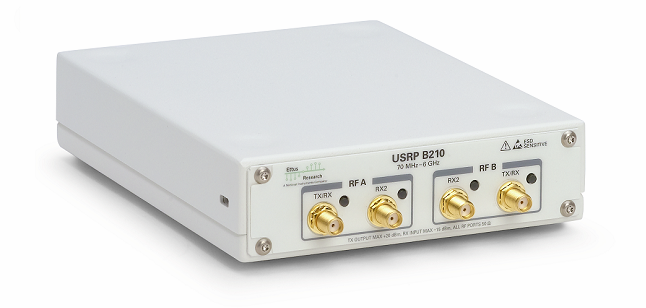
\includegraphics[width=0.7\linewidth]{figures/b210}
        \caption{USRP B210}
        \label{fig:b210}
    \end{subfigure}
    \begin{subfigure}[htb]{0.45\textwidth}
        \centering
        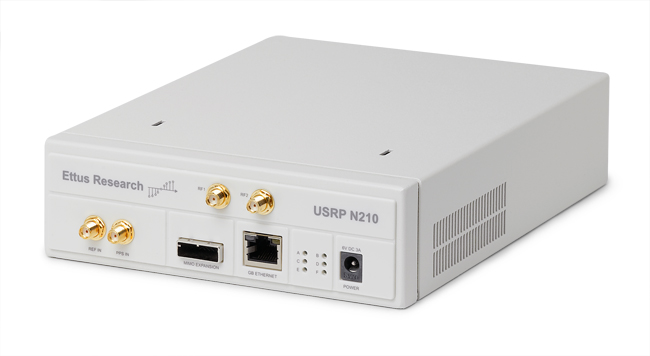
\includegraphics[width=0.7\linewidth]{figures/n210}
        \caption{USRP N210}
        \label{fig:n210}
    \end{subfigure}
    \begin{subfigure}[htb]{0.5\textwidth}
        \centering
        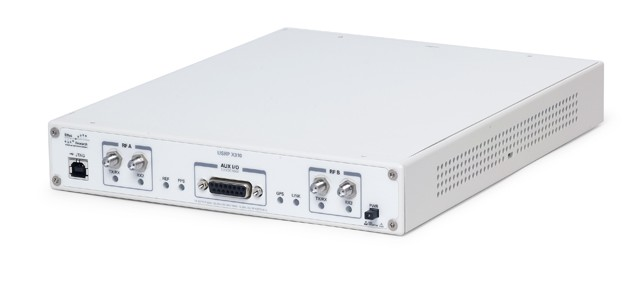
\includegraphics[width=0.7\linewidth]{figures/x310}
        \caption{USRP X300}
        \label{fig:x300}
    \end{subfigure}
    \begin{subfigure}[htb]{0.4\textwidth}
        \centering
        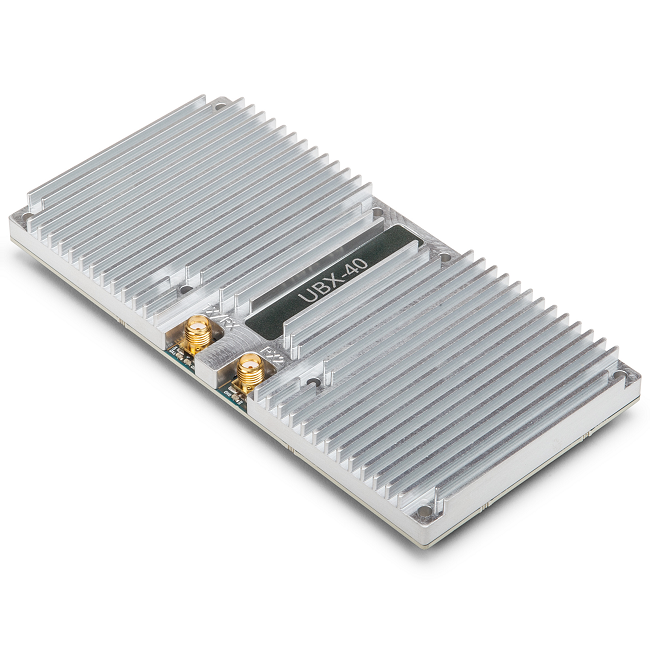
\includegraphics[width=0.6\linewidth]{figures/UBX40}
        \caption{UBX-40 daughterboard}
        \label{fig:UBX}
    \end{subfigure}
    \caption{\ac{USRP} Devices used in the complete DySpan challenge setup}
    \label{fig:ettus}
\end{figure}

For this thesis, the \ac{SU} implementation is reproduced, for which the N210 as transmitter and the B210 as receiver are used.

\section{Machine Learning models in Python and Jupyter}
\begin{figure}[!h]
    \centering
    \begin{subfigure}[htb]{0.45\textwidth}
        \centering
        
\includegraphics[width=\linewidth]{figures/python_logo}
        \label{fig:python}
    \end{subfigure}
    \begin{subfigure}[htb]{0.45\textwidth}
        \centering
        
\includegraphics[width=\linewidth]{figures/jupyter_logo}
        \label{fig:jupyter}
    \end{subfigure}
    \caption{Python and Jupyter logos}
    \label{fig:python_jupyter}
\end{figure}
For the learning part of this work, the focus on the implementation was given to a couple of popular Python libraries that have been effective when dealing with \ac{ML} problems: scikit-learn \cite{SKLEARN} and keras \cite{KERAS}. This libraries were chosen because of the simplicity of their prototyping as well as their effectiveness when providing an implementation that suits the \ac{ML} needs by returning fully trained models with exceptional prediction accuracy, and are described in more detail in the following sections. Additionally, the fact that these libraries are written in Python raises interest because this means that they interface optimally with GNURadio, making the inclussion of these libraries transparent, and having the perks of Python such as easy debugging and extensibility.\\

As for model testing and visualization, Jupyter notebooks \cite{Jupyter} have been used and are presented as part of the code repository of this thesis. What Jupyter provides is an open-source web application in which a number of interpreters for languages such as Python, R, Julia and Scala are embedded, allowing the creation and sharing of interactive register that contains code lines and excecution output along with visualization fields for plots and graphs and documentation in markdown, in what is called \emph{literate programming}. These notebooks can be shared in multiple formats, such as the native notebook format (for further modification of its contents), as well as HTML, \LaTeX{} and PDF (generated with \LaTeX). Moreover, it is nicely integrated with GitHub, so that the notebook can be visualized in the webpage of a remote repository without the need of conversion.\\

Jupyter is the continuation of a long effort for supporting interactive Python interpreters - the IPython Project \cite{IPython}. It has had a bast adoption in the last few years, such that even complete books have been written only using Jupyter as their interface for text editing and code examples. One of the main sources used for this work \cite{Andreas} is one example of such.

\subsection{Scikit-learn}
\begin{figure}[!h]
    \centering
    
\includegraphics[width=0.4\linewidth]{figures/sklearn_logo}
    \label{fig:sklearn_logo}
    \caption{Scikit-learn logo}
\end{figure}
Scikit-learn, formerly scikits.learn and also known as sklearn, is \ac{ML} library that features an abundance of algorithms for supervised and unsupervised algorithms, including the ones described in section~\ref{ch:ml_algs}. This library came as a result from a \emph{Google Summer of Code} project as a third party extension to SciPy, from where it gets its name. This library was used in this thesis for all the learning based on the extracted features listed in section~\ref{ch:features}.

\subsection{Keras}
\begin{figure}[!h]
    \centering
    
\includegraphics[width=0.5\linewidth]{figures/keras_logo}
    \label{fig:keras_logo}
    \caption{Keras logo}
\end{figure}
Keras is a high-level neural networks API written in Python that uses TensorFlow \cite{TensorFlow}, CNTK \cite{CNTK} or Theano \cite{Theano} as a backend. The way it is written in a way that allows datascientist to prototype and experiment fast. As per its documentation \cite{KERAS}:\emph{"being able to go from idea to result with the least possible delay is key to doing good research"}, and Keras certainly intends to keep the coding part as simple as possible for the designer to focus on the idea and not the programming of it. For this, it presents and API that is:

\begin{itemize}
    \item User-friendly: with ease for writing, reading and understanding.
    \item Modular: models have a clear begin and end, and they can be easily connected with other models with low to none restrictions.
    \item  Extendible: new functionalities and features are easily added to the mainstream, and the existing codebase is well-documented and exemplified.
\end{itemize}

For this project, Keras is used for convolutional neural networks implementation, using Tensorflow (with GPU support) as a backend.

\section{Data set Generation}
This part of the work regards the steps taken in order to have the data ready for the \ac{ML} algorithms to learn from it. It covers the testbed setup, the raw data (I/Q samples) measurement, and the data preprocessing.
\subsection{Measure Campaign}
The first step taken was to set up the \ac{PU} communication link over the air, and recording the raw samples just as the \ac{SU} would be able to "hear" them. The measurement setup is shown in Fig~\ref{fig:measurement}, where two parts are labeled separately.

\begin{figure}[!htb]
    \centering
    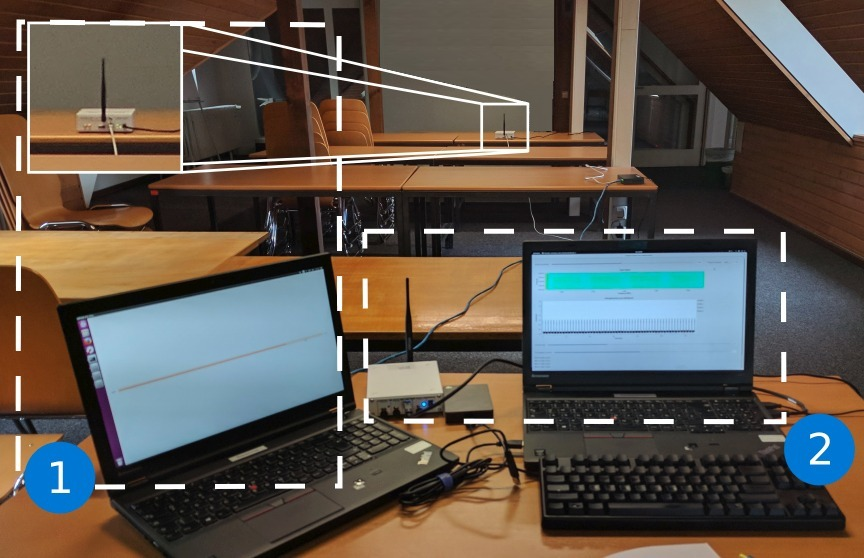
\includegraphics[width=0.5\linewidth]{figures/mod}
    \label{fig:measurement}
    \caption{Measurement Setup}
\end{figure}

The part labeled with \textcircled{1} regards the transmission part, which is going to be sending frames over the air in ten different fashions, described in Table~\ref{table:scenarios}.  The host machine in this part has the connection to the database, from where the information frames are extracted and put as payload of the transmitted frames. Additionally, the GNURadio flowgraph that generates the signal, which can be seen in Fig~\ref{fig:PU_flowgraph}, is also hosted and run from this computer. A summary of the path that a frame travels from the database until the transmitter is as follows: in Fig.~\ref{fig:PU_flowgraph} it can be seen that a connection to the database is done in the "Cmd pktgen" block, which is in charge of retreiving the information frames from the database, in form of \ac{PDU}, and feeding them into the signal processing blocks. After converting the \ac{PDU} into a tagged stream (a stream of data that has metadata attached to it in form of tags), the stream flows into the \ac{OFDM} transmitter block, which is a hierarchical block that allocates the carriers for an \ac{OFDM} transmission, applies a \ac{FFT} to them, and appends a cyclic prefix.

\begin{figure}[!htb]
    \centering
    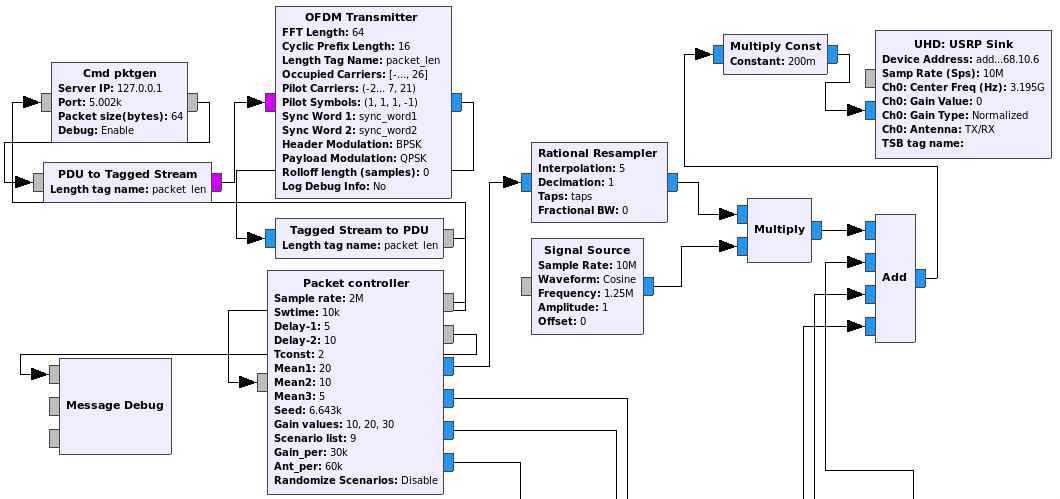
\includegraphics[width=\textwidth]{figures/PU_flowgraph}
    \label{fig:PU_flowgraph}
    \caption{\ac{PU} GNURadio flowgraph}
\end{figure}

\subsection{Feature Engineering}\label{ch:features}
\subsection{Spectrograms generation}

  \acresetall
\chapter{Evaluation and Results}\label{ch:evaluation}
In this chapter, a benchmark of the analyzed algorithms is presented, based on dataset size and complexity. For the first part, the algorithms used for supervised learning are presented, for which an analysis of the different complexities used is made. From the benchmark, the trained models with the best performance are saved and then used in the live implementation presented in chapter~\ref{ch:live}. The process of saving trained models for later use is called \emph{model persistence}.

\section{Performance metrics}\label{ch:performance}

The impact of the dataset size on the algorithm performance is of special interest. Given that the data recorded using the procedure described in section~\ref{ch:measure} has a fixed size, this analysis was performed by slicing the resulting feature extraction files to emulate different dataset sizes. It is important to notice that only "slicing", in order to emulate smaller datasets, and not "repeating samples", for emulation of bigger datasets, has a significant impact on the performance, as noted in section~\ref{ch:size}. This is due to the fact that repeated samples present no new information to the model, and there is nothing new to learn from them.

The dataset is, then, sliced into four different sizes:

\begin{itemize}
    \item Small dataset (S): is one fourth (1/4) of the original dataset
    \item Medium dataset (M): is one third (1/3) of the original dataset
    \item Large dataset (L): is half (1/2) of the original dataset
    \item Extra Large dataset (XL): the whole set of features extracted as recorded from the signals over the air.
\end{itemize}

Furthermore, a benchmark of the learning algorithms is made based on variations on their complexities. Each algorithm has different ways to represent its own complexity, and this has a significant impact on its overall performance. The \ac{ML} algorithms used in this analysis are K-nearest neighbors, \ac{SVM} and binary tree classification. Their complexities are set as follows:

\begin{itemize}
    \item K-nearest neighbors: the complexity of this algorithm is set by the amount of neighbors that are considered in order to make a classification decision. For the benchmark, different models were trained using from 1 neighbor up to 200 neighbors
    \item \ac{SVM}: this algorithm allows the designer to select the type of kernel that is used during the learning process. The function of the kernel is to generate internally non-linear transformations over the input data while still behaving as a linear classificator. For this work, the \ac{RBF} is used as a kernel because of its known good performance on multiclass classification problems at the cost of longer training times. The complexity of this model is then set by providing different values to the '\(\gamma\)' parameter of this \ac{RBF} kernel, whose kernel function is:
        \begin{equation}
            \text{exp}(-\gamma || x - x'||^2
        \end{equation}
        For this work, values of \(\gamma=2^{-15}, 2^{-13}, 2^{-11}, 2^{-9}, 2^{-7}, 2^{-5}, 2^{-3}, 2^{-1}, 2^{1} \text{ and }2^{3} \) are used.


    \item Decision Trees: in this model, the complexity is ruled by the depth of the decision branch. Here, depths from 1 up to 500 are used.
\end{itemize}

Moreover, it is also interesting to determine how the models behave when the features have been scaled. A first glance at the impact of a scaler is presented by using the StandardScaler() from SKlearn, which simply removes the mean of the features and scales them to unit variance. A side-by-side comparison of model performance when trained with unscaled features vs.scaled features is shown as a result of the benchmark. The results are depicted in Figs~\ref{fig:knn}, \ref{fig:dtc} and \ref{fig:svc}.

\begin{figure}[!htb]
    \centering
    \begin{subfigure}[t]{0.49\textwidth}
        \centering
        \begin{tikzpicture}[scale=0.8]
            \begin{axis}[
                xlabel={\# of Neighbors},
                ylabel={Accuracy},
                legend style={at={(1.2,1.20)},
                    anchor=north,legend columns=-1},
                  ]
                \addplot[color=blue] table [x=N, y=S, col sep=comma, mark=none] {data/knn_accs.csv};
                \addplot[color=red] table [x=N, y=M, col sep=comma, mark=none] {data/knn_accs.csv};
                \addplot[color=green] table [x=N, y=L, col sep=comma, mark=none] {data/knn_accs.csv};
                \addplot[color=orange] table [x=N, y=XL, col sep=comma, mark=none] {data/knn_accs.csv};
                \legend{Dataset S, Dataset M, Dataset L, Dataset XL}
        \end{axis}
        \end{tikzpicture}
        \caption{Accuracy with unscaled features}
        \label{fig:knn_accs_scaled}
    \end{subfigure}
        \hfill
    \begin{subfigure}[t]{0.49\textwidth}
        \centering
        \begin{tikzpicture}[scale=0.8]
            \begin{axis}[
                xlabel={\# of Neighbors},
                ylabel={Accuracy},
                  ]
                \addplot[color=blue] table [x=N, y=S, col sep=comma, mark=none] {data/knn_accs_scaled.csv};
                \addplot[color=red] table [x=N, y=M, col sep=comma, mark=none] {data/knn_accs_scaled.csv};
                \addplot[color=green] table [x=N, y=L, col sep=comma, mark=none] {data/knn_accs_scaled.csv};
                \addplot[color=orange] table [x=N, y=XL, col sep=comma, mark=none] {data/knn_accs_scaled.csv};
        \end{axis}
        \end{tikzpicture}
        \caption{Accuracy with scaled features}
        \label{fig:knn_accs_scaled}
    \end{subfigure}
    \begin{subfigure}[t]{0.49\textwidth}
        \centering
        \begin{tikzpicture}[scale=0.8]
            \begin{axis}[
                xlabel={\# of Neighbors},
                ylabel={Training time (s)},
                  ]
                \addplot[color=blue]table [x=N, y=S, col sep=comma, mark=none] {data/knn_fit_times.csv};
                \addplot[color=red] table [x=N, y=M, col sep=comma, mark=none] {data/knn_fit_times.csv};
                \addplot[color=green] table [x=N, y=L, col sep=comma, mark=none] {data/knn_fit_times.csv};
                \addplot[color=orange] table [x=N, y=XL, col sep=comma, mark=none] {data/knn_fit_times.csv};
        \end{axis}
        \end{tikzpicture}
        \caption{Training times with unscaled features}
        \label{fig:knn_fit_times}
    \end{subfigure}
    \centering
        \hfill
    \begin{subfigure}[t]{0.49\textwidth}
        \centering
        \begin{tikzpicture}[scale=0.8]
            \begin{axis}[
                xlabel={\# of Neighbors},
                ylabel={Training time (s)},
                  ]
                \addplot[color=blue]table [x=N, y=S, col sep=comma, mark=none] {data/knn_fit_times_scaled.csv};
                \addplot[color=red] table [x=N, y=M, col sep=comma, mark=none] {data/knn_fit_times_scaled.csv};
                \addplot[color=green] table [x=N, y=L, col sep=comma, mark=none] {data/knn_fit_times_scaled.csv};
                \addplot[color=orange] table [x=N, y=XL, col sep=comma, mark=none] {data/knn_fit_times_scaled.csv};
        \end{axis}
        \end{tikzpicture}
        \caption{Training times with scaled features}
        \label{fig:knn_fit_times_scaled}
    \end{subfigure}
    \begin{subfigure}[t]{0.49\textwidth}
        \centering
        \begin{tikzpicture}[scale=0.8]
            \begin{axis}[
                xlabel={\# of Neighbors},
                ylabel={Prediction time (s)},
                  ]
                \addplot[color=blue]table [x=N, y=S, col sep=comma, mark=none] {data/knn_pred_times.csv};
                \addplot[color=red] table [x=N, y=M, col sep=comma, mark=none] {data/knn_pred_times.csv};
                \addplot[color=green] table [x=N, y=L, col sep=comma, mark=none] {data/knn_pred_times.csv};
                \addplot[color=orange] table [x=N, y=XL, col sep=comma, mark=none] {data/knn_pred_times.csv};
        \end{axis}
        \end{tikzpicture}
        \caption{Prediction times with unscaled features}
        \label{fig:knn_pred_times}
    \end{subfigure}
    \centering
        \hfill
    \begin{subfigure}[t]{0.49\textwidth}
        \centering
        \begin{tikzpicture}[scale=0.8]
            \begin{axis}[
                xlabel={\# of Neighbors},
                ylabel={Prediction time (s)},
                  ]
                \addplot[color=blue]table [x=N, y=S, col sep=comma, mark=none] {data/knn_pred_times_scaled.csv};
                \addplot[color=red] table [x=N, y=M, col sep=comma, mark=none] {data/knn_pred_times_scaled.csv};
                \addplot[color=green] table [x=N, y=L, col sep=comma, mark=none] {data/knn_pred_times_scaled.csv};
                \addplot[color=orange] table [x=N, y=XL, col sep=comma, mark=none] {data/knn_pred_times_scaled.csv};
        \end{axis}
        \end{tikzpicture}
        \caption{Prediction times with scaled features}
        \label{fig:knn_pred_times}
    \end{subfigure}
    \caption{Metrics for K-Nearest Neighbors}
    \label{fig:knn}
\end{figure}

\begin{figure}[!htb]
    \centering
    \begin{subfigure}[t]{0.49\textwidth}
        \centering
        \begin{tikzpicture}[scale=0.8]
            \begin{axis}[
                xlabel={Tree depth},
                ylabel={Accuracy},
                legend style={at={(1.2,1.20)},
                    anchor=north,legend columns=-1},
                  ]
                \addplot[color=blue] table [x=N, y=S, col sep=comma, mark=none] {data/dtc_accs.csv};
                \addplot[color=red] table [x=N, y=M, col sep=comma, mark=none] {data/dtc_accs.csv};
                \addplot[color=green] table [x=N, y=L, col sep=comma, mark=none] {data/dtc_accs.csv};
                \addplot[color=orange] table [x=N, y=XL, col sep=comma, mark=none] {data/dtc_accs.csv};
                \legend{Dataset S, Dataset M, Dataset L, Dataset XL}
        \end{axis}
        \end{tikzpicture}
        \caption{Accuracy with unscaled features}
        \label{fig:dtc_accs_scaled}
    \end{subfigure}
        \hfill
    \begin{subfigure}[t]{0.49\textwidth}
        \centering
        \begin{tikzpicture}[scale=0.8]
            \begin{axis}[
                xlabel={Tree depth},
                ylabel={Accuracy},
                  ]
                \addplot[color=blue] table [x=N, y=S, col sep=comma, mark=none] {data/dtc_accs_scaled.csv};
                \addplot[color=red] table [x=N, y=M, col sep=comma, mark=none] {data/dtc_accs_scaled.csv};
                \addplot[color=green] table [x=N, y=L, col sep=comma, mark=none] {data/dtc_accs_scaled.csv};
                \addplot[color=orange] table [x=N, y=XL, col sep=comma, mark=none] {data/dtc_accs_scaled.csv};
        \end{axis}
        \end{tikzpicture}
        \caption{Accuracy with scaled features}
        \label{fig:dtc_accs_scaled}
    \end{subfigure}
    \begin{subfigure}[t]{0.49\textwidth}
        \centering
        \begin{tikzpicture}[scale=0.8]
            \begin{axis}[
                xlabel={Tree depth},
                ylabel={Training time (s)},
                  ]
                \addplot[color=blue]table [x=N, y=S, col sep=comma, mark=none] {data/dtc_fit_times.csv};
                \addplot[color=red] table [x=N, y=M, col sep=comma, mark=none] {data/dtc_fit_times.csv};
                \addplot[color=green] table [x=N, y=L, col sep=comma, mark=none] {data/dtc_fit_times.csv};
                \addplot[color=orange] table [x=N, y=XL, col sep=comma, mark=none] {data/dtc_fit_times.csv};
        \end{axis}
        \end{tikzpicture}
        \caption{Training times with unscaled features}
        \label{fig:dtc_fit_times}
    \end{subfigure}
    \centering
        \hfill
    \begin{subfigure}[t]{0.49\textwidth}
        \centering
        \begin{tikzpicture}[scale=0.8]
            \begin{axis}[
                xlabel={Tree depth},
                ylabel={Training time (s)},
                  ]
                \addplot[color=blue]table [x=N, y=S, col sep=comma, mark=none] {data/dtc_fit_times_scaled.csv};
                \addplot[color=red] table [x=N, y=M, col sep=comma, mark=none] {data/dtc_fit_times_scaled.csv};
                \addplot[color=green] table [x=N, y=L, col sep=comma, mark=none] {data/dtc_fit_times_scaled.csv};
                \addplot[color=orange] table [x=N, y=XL, col sep=comma, mark=none] {data/dtc_fit_times_scaled.csv};
        \end{axis}
        \end{tikzpicture}
        \caption{Training times with scaled features}
        \label{fig:dtc_fit_times_scaled}
    \end{subfigure}
    \begin{subfigure}[t]{0.49\textwidth}
        \centering
        \begin{tikzpicture}[scale=0.8]
            \begin{axis}[
                xlabel={Tree depth},
                ylabel={Prediction time (s)},
                  ]
                \addplot[color=blue]table [x=N, y=S, col sep=comma, mark=none] {data/dtc_pred_times.csv};
                \addplot[color=red] table [x=N, y=M, col sep=comma, mark=none] {data/dtc_pred_times.csv};
                \addplot[color=green] table [x=N, y=L, col sep=comma, mark=none] {data/dtc_pred_times.csv};
                \addplot[color=orange] table [x=N, y=XL, col sep=comma, mark=none] {data/dtc_pred_times.csv};
        \end{axis}
        \end{tikzpicture}
        \caption{Prediction times with unscaled features}
        \label{fig:dtc_pred_times}
    \end{subfigure}
    \centering
        \hfill
    \begin{subfigure}[t]{0.49\textwidth}
        \centering
        \begin{tikzpicture}[scale=0.8]
            \begin{axis}[
                xlabel={Tree depth},
                ylabel={Prediction time (s)},
                  ]
                \addplot[color=blue]table [x=N, y=S, col sep=comma, mark=none] {data/dtc_pred_times_scaled.csv};
                \addplot[color=red] table [x=N, y=M, col sep=comma, mark=none] {data/dtc_pred_times_scaled.csv};
                \addplot[color=green] table [x=N, y=L, col sep=comma, mark=none] {data/dtc_pred_times_scaled.csv};
                \addplot[color=orange] table [x=N, y=XL, col sep=comma, mark=none] {data/dtc_pred_times_scaled.csv};
        \end{axis}
        \end{tikzpicture}
        \caption{Prediction times with scaled features}
        \label{fig:dtc_pred_times}
    \end{subfigure}
    \caption{Metrics for the decision tree classifier}
    \label{fig:dtc}
\end{figure}



\begin{figure}[!htb]
    \centering
    \begin{subfigure}[t]{0.49\textwidth}
        \centering
        \begin{tikzpicture}[scale=0.8]
            \begin{axis}[
                    xlabel={\(\gamma\) for \ac{RBF} kernel - \ac{SVM}},
                ylabel={Accuracy},
                legend style={at={(1.2,1.20)},
                    anchor=north,legend columns=-1},
                  ]
                \addplot[color=blue] table [x=N, y=S, col sep=comma, mark=none] {data/svc_accs.csv};
                \addplot[color=red] table [x=N, y=M, col sep=comma, mark=none] {data/svc_accs.csv};
                \addplot[color=green] table [x=N, y=L, col sep=comma, mark=none] {data/svc_accs.csv};
                \addplot[color=orange] table [x=N, y=XL, col sep=comma, mark=none] {data/svc_accs.csv};
                \legend{Dataset S, Dataset M, Dataset L, Dataset XL}
        \end{axis}
        \end{tikzpicture}
        \caption{Accuracy with unscaled features}
        \label{fig:svc_accs_scaled}
    \end{subfigure}
        \hfill
    \begin{subfigure}[t]{0.49\textwidth}
        \centering
        \begin{tikzpicture}[scale=0.8]
            \begin{axis}[
                    xlabel={\(\gamma\) for \ac{RBF} kernel - \ac{SVM}},
                ylabel={Accuracy},
                  ]
                \addplot[color=blue] table [x=N, y=S, col sep=comma, mark=none] {data/svc_accs_scaled.csv};
                \addplot[color=red] table [x=N, y=M, col sep=comma, mark=none] {data/svc_accs_scaled.csv};
                \addplot[color=green] table [x=N, y=L, col sep=comma, mark=none] {data/svc_accs_scaled.csv};
                \addplot[color=orange] table [x=N, y=XL, col sep=comma, mark=none] {data/svc_accs_scaled.csv};
        \end{axis}
        \end{tikzpicture}
        \caption{Accuracy with scaled features}
        \label{fig:svc_accs_scaled}
    \end{subfigure}
    \begin{subfigure}[t]{0.49\textwidth}
        \centering
        \begin{tikzpicture}[scale=0.8]
            \begin{axis}[
                    xlabel={\(\gamma\) for \ac{RBF} kernel - \ac{SVM}},
                ylabel={Training time (s)},
                  ]
                \addplot[color=blue]table [x=N, y=S, col sep=comma, mark=none] {data/svc_fit_times.csv};
                \addplot[color=red] table [x=N, y=M, col sep=comma, mark=none] {data/svc_fit_times.csv};
                \addplot[color=green] table [x=N, y=L, col sep=comma, mark=none] {data/svc_fit_times.csv};
                \addplot[color=orange] table [x=N, y=XL, col sep=comma, mark=none] {data/svc_fit_times.csv};
        \end{axis}
        \end{tikzpicture}
        \caption{Training times with unscaled features}
        \label{fig:svc_fit_times}
    \end{subfigure}
    \centering
        \hfill
    \begin{subfigure}[t]{0.49\textwidth}
        \centering
        \begin{tikzpicture}[scale=0.8]
            \begin{axis}[
                    xlabel={\(\gamma\) for \ac{RBF} kernel - \ac{SVM}},
                ylabel={Training time (s)},
                  ]
                \addplot[color=blue]table [x=N, y=S, col sep=comma, mark=none] {data/svc_fit_times_scaled.csv};
                \addplot[color=red] table [x=N, y=M, col sep=comma, mark=none] {data/svc_fit_times_scaled.csv};
                \addplot[color=green] table [x=N, y=L, col sep=comma, mark=none] {data/svc_fit_times_scaled.csv};
                \addplot[color=orange] table [x=N, y=XL, col sep=comma, mark=none] {data/svc_fit_times_scaled.csv};
        \end{axis}
        \end{tikzpicture}
        \caption{Training times with scaled features}
        \label{fig:svc_fit_times_scaled}
    \end{subfigure}
    \begin{subfigure}[t]{0.49\textwidth}
        \centering
        \begin{tikzpicture}[scale=0.8]
            \begin{axis}[
                    xlabel={\(\gamma\) for \ac{RBF} kernel - \ac{SVM}},
                ylabel={Prediction time (s)},
                  ]
                \addplot[color=blue]table [x=N, y=S, col sep=comma, mark=none] {data/svc_pred_times.csv};
                \addplot[color=red] table [x=N, y=M, col sep=comma, mark=none] {data/svc_pred_times.csv};
                \addplot[color=green] table [x=N, y=L, col sep=comma, mark=none] {data/svc_pred_times.csv};
                \addplot[color=orange] table [x=N, y=XL, col sep=comma, mark=none] {data/svc_pred_times.csv};
        \end{axis}
        \end{tikzpicture}
        \caption{Prediction times with unscaled features}
        \label{fig:svc_pred_times}
    \end{subfigure}
    \centering
        \hfill
    \begin{subfigure}[t]{0.49\textwidth}
        \centering
        \begin{tikzpicture}[scale=0.8]
            \begin{axis}[
                    xlabel={\(\gamma\) for \ac{RBF} kernel - \ac{SVM}},
                ylabel={Prediction time (s)},
                  ]
                \addplot[color=blue]table [x=N, y=S, col sep=comma, mark=none] {data/svc_pred_times_scaled.csv};
                \addplot[color=red] table [x=N, y=M, col sep=comma, mark=none] {data/svc_pred_times_scaled.csv};
                \addplot[color=green] table [x=N, y=L, col sep=comma, mark=none] {data/svc_pred_times_scaled.csv};
                \addplot[color=orange] table [x=N, y=XL, col sep=comma, mark=none] {data/svc_pred_times_scaled.csv};
        \end{axis}
        \end{tikzpicture}
        \caption{Prediction times with scaled features}
        \label{fig:svc_pred_times}
    \end{subfigure}
    \caption{Metrics for \ac{SVM}}
    \label{fig:svc}
\end{figure}




%\begin{figure}[!htb]
    %\centering
    %\begin{subfigure}[htb]{0.49\textwidth}
        %\centering
        %\includestandalone[width=\linewidth]{figures/knn_accs}
        %\label{fig:knn_accs}
    %\end{subfigure}
    %\begin{subfigure}[htb]{0.49\textwidth}
        %\centering
        %\includestandalone[width=\linewidth]{figures/knn_accs_scaled}
        %\caption{Accuracy with scaled features}
        %\label{fig:knn_accs_scaled}
    %\end{subfigure}\\
    %\begin{subfigure}[htb]{0.49\textwidth}
        %\centering
        %\includestandalone[width=\linewidth]{figures/knn_fit_times}
        %\caption{Training times with unscaled features}
        %\label{fig:knn_fit_times}
    %\end{subfigure}
    %\begin{subfigure}[htb]{0.49\textwidth}
        %\centering
        %\includestandalone[width=\linewidth]{figures/knn_fit_times_scaled}
        %\caption{Training times with scaled features}
        %\label{fig:knn_fit_times_scaled}
    %\end{subfigure}\\
    %\begin{subfigure}[htb]{0.49\textwidth}
        %\centering
        %\includestandalone[width=\linewidth]{figures/knn_pred_times}
        %\caption{Prediction times with unscaled features}
        %\label{fig:knn_pred_times}
    %\end{subfigure}
    %\begin{subfigure}[htb]{0.49\textwidth}
        %\centering
        %\includestandalone[width=\linewidth]{figures/knn_pred_times_scaled}
        %\caption{Prediction times with scaled features}
        %\label{fig:knn_pred_times_scaled}
    %\end{subfigure}
    %\caption{K-nearest Neighbors}
    %\label{fig:knn}
%\end{figure}

%\begin{figure}[!htb]
    %\centering
    %\begin{subfigure}[htb]{0.49\textwidth}
        %\centering
        %\includestandalone[width=\linewidth]{figures/dtc_accs}
        %\caption{Accuracy with unscaled features}
        %\label{fig:dtc_accs}
    %\end{subfigure}
    %\begin{subfigure}[htb]{0.49\textwidth}
        %\centering
        %\includestandalone[width=\linewidth]{figures/dtc_accs_scaled}
        %\caption{Accuracy with scaled features}
        %\label{fig:dtc_accs_scaled}
    %\end{subfigure}
    %\begin{subfigure}[htb]{0.49\textwidth}
        %\centering
        %\includestandalone[width=\linewidth]{figures/dtc_fit_times}
        %\caption{Training times with unscaled features}
        %\label{fig:dtc_fit_times}
    %\end{subfigure}
    %\begin{subfigure}[htb]{0.49\textwidth}
        %\centering
        %\includestandalone[width=\linewidth]{figures/dtc_fit_times_scaled}
        %\caption{Training times with scaled features}
        %\label{fig:dtc_fit_times_scaled}
    %\end{subfigure}
    %\begin{subfigure}[htb]{0.49\textwidth}
        %\centering
        %\includestandalone[width=\linewidth]{figures/dtc_pred_times}
        %\caption{Prediction times with unscaled features}
        %\label{fig:dtc_pred_times}
    %\end{subfigure}
    %\begin{subfigure}[htb]{0.49\textwidth}
        %\centering
        %\includestandalone[width=\linewidth]{figures/dtc_pred_times_scaled}
        %\caption{Prediction times with scaled features}
        %\label{fig:dtc_pred_times_scaled}
    %\end{subfigure}
    %\caption{Decision Trees}
    %\label{fig:dtc}
%\end{figure}

%\begin{figure}
    %\centering
    %\begin{subfigure}[htb]{0.49\textwidth}
        %\centering
        %\includestandalone[width=\linewidth]{figures/svc_accs}
        %\caption{Accuracy with unscaled features}
        %\label{fig:svc_accs}
    %\end{subfigure}
    %\begin{subfigure}[htb]{0.49\textwidth}
        %\centering
        %\includestandalone[width=\linewidth]{figures/svc_accs_scaled}
        %\caption{Accuracy with scaled features}
        %\label{fig:svc_accs_scaled}
    %\end{subfigure}
    %\begin{subfigure}[b]{0.49\textwidth}
        %\centering
        %\includestandalone[width=\linewidth]{figures/svc_fit_times}
        %\caption{Training times with unscaled features}
        %\label{fig:svc_fit_times}
    %\end{subfigure}
    %\begin{subfigure}[b]{0.49\textwidth}
        %\centering
        %\includestandalone[width=\linewidth]{figures/svc_fit_times_scaled}
        %\caption{Training times with scaled features}
        %\label{fig:svc_fit_times_scaled}
    %\end{subfigure}
    %\begin{subfigure}[b]{0.49\textwidth}
        %\centering
        %\includestandalone[width=\linewidth]{figures/svc_pred_times}
        %\caption{Prediction times with unscaled features}
        %\label{fig:svc_pred_times}
    %\end{subfigure}
    %\begin{subfigure}[b]{0.49\textwidth}
        %\centering
        %\includestandalone[width=\linewidth]{figures/svc_pred_times_scaled}
        %\caption{Prediction times with scaled features}
        %\label{fig:dtc_pred_times_scaled}
    %\end{subfigure}
    %\caption{Support Vector Machines}
    %\label{fig:svc}
%\end{figure}

From Figs~\ref{fig:knn}, \ref{fig:dtc} and \ref{fig:svc} a couple of conclusions can be extracted. First, it is seen that the accuracy of the model increases as more data is taken into consideration, which is well according to the theory and serves as a catalyst for applying the same implementation with more data as proposed in chapter~\ref{ch:conclusions}. Furthermore, three different behaviors are appreciated:

\begin{itemize}
    \item As complexity increases, the K-nearest neighbors algorithm shows a decrease on its overall accuracy, which is an indication that the model is over-generalizing, and suggests that with such a complexity (above few neighbors), the model is starting to loosely classify scenarios, allowing more samples to be misclassified, and is set to perform badly if unknown samples are feed to it, as its capabilities for generalization are in decay. Moreover, the prediction times for the highest level of complexity are already about two times greater than the second highest, making high K-nearest neighbors complexity not suitable for live implementations. Furthermore, this model shows both a reduction in accuracy and an increase on prediction time when the features have been scaled, which simply states that the model performs well without further data preprocessing right after the feature extraction.
    \item The decision tree model shows a steady increase on its accuracy as complexity increases, without reaching a clear overfitting state. Complexity has a clear effect on the training times, but it is still in the range of the milliseconds - being a process done only once, this does not affect dramatically the model selection and does not close the possibility of increasing the complexity for this specific use case. This can also be backed by the fact that the prediction times seem to stay constant with this increase. Interestingly, not only the training times are reduced after scaling, but also the prediction times are drastically improved, reaching about 10x faster predictions using the standard scaler. With comparable accuracy, scaling the features seems like a prospect procedure when this model is used in time demanding or live implementations.
        The low accuracy of this model when a depth=2 does not come as a surprise. As the classification is done based on \emph{if-then} steps, having such a short depth can only provide four possible predicted values, as it can be seen in the extracted tree shown in Fig~\ref{fig:dt_2}. This model is generated as an experimental exercise to show this behavior, and to make the statement that the depth of the tree has to be able to generate at least as many answers as classes of the problem, which in this specific use case is achieved with a depth=\(2^4 > 10\). Graphical representations of complex decision trees are easily generated, but they become overwhelming for them to be shown in this print. The procedure to generate these trees is explained in the development notebook of this thesis \cite{repo:cognitive_radio_ml}.

\begin{figure}[!htb]
    \centering
      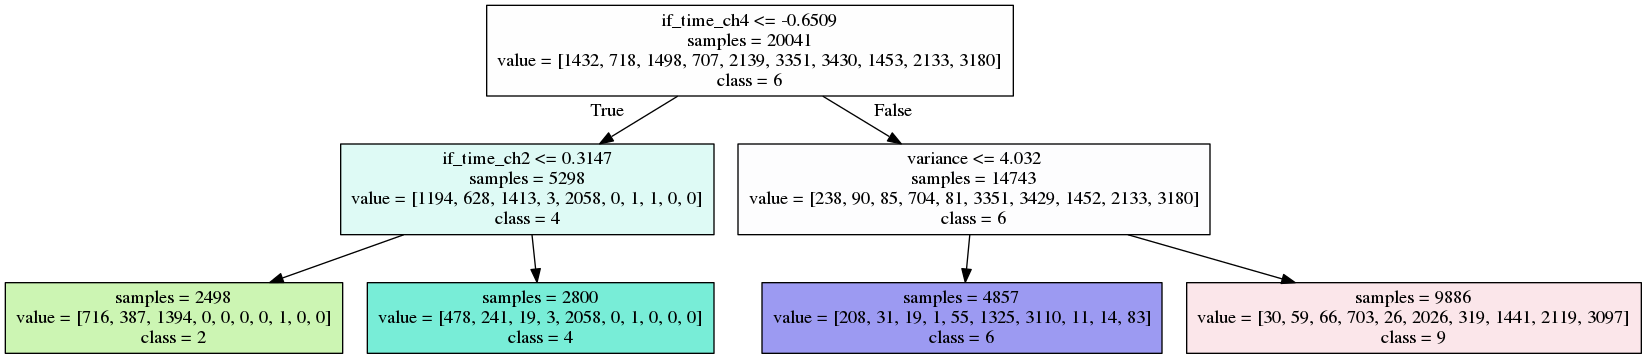
\includegraphics[width=\textwidth]{figures/dt_2}
      \caption{Extracted representation of a trained decision tree with depth=2}
      \label{fig:dt_2}
\end{figure}

    \item the \ac{SVM} show a clear tendency to improve as complexity is increased only if the data has been scaled, which indicates the sensitivity of this model to unscaled data.  However, the best accuracy of this model is still below the accuracies of the other models regarded in this benchmark. Additionally, the training and prediction times exceed dramatically the times achieved with the other models, being about 8000 times longer for training and around 500 times longer for prediction. The fact that this model is that slow will definitely affect considerably the performance of real-time implementations, an aspect that is crucial in systems such as cognitive radio, and therefore would not be recommended for that type of implementations.
\end{itemize}

\section{Scenario Classification}
Besides of the general performance that the learning models have in regard to the whole testing set, it is paramount to determine how good they perform by classifying each of the specific scenarios of Table~\ref{table:scenarios}. To assess this, confusion matrices are used to determine the number of correctly classified scenarios, along with the false positives and false negatives. On this analysis, it is only of interest the number of correctly classified scenarios, and any misclassification affects the implementation equally, regardless of its type. Moreover, in section~\ref{ch:performance} can be seen that each algorithm behaves differently in terms not only of accuracy, but also in training time and prediction time. As the models are trained only once, the "training time" does not play a role in the model selection for this work, as it does not have any repercussion on the performance of the model when new values are applied to it. Therefore, "prediction time" and "accuracy" are metrics of quality that are considered for these models on its selection to be applied on real-time scenarios.\\

Confusion matrices show how each of the samples from the data set are classified for a given model. As a matter of illustration, a side by side comparison for the worst-performing vs. the best-performing model, with respect to accuracy, is given in Fig~\ref{fig:confusionknn}, \ref{fig:confusiondtc} and \ref{fig:confusionsvc}. The complete set of confusion matrices, corresponding to every trained model, can be found in the development notebook for this work \cite{repo:cognitive_radio_ml}.


\begin{figure}[!htb]
    \captionsetup[subfigure]{justification=centering}
    \centering
    \begin{subfigure}[htb]{0.49\textwidth}
        \centering
        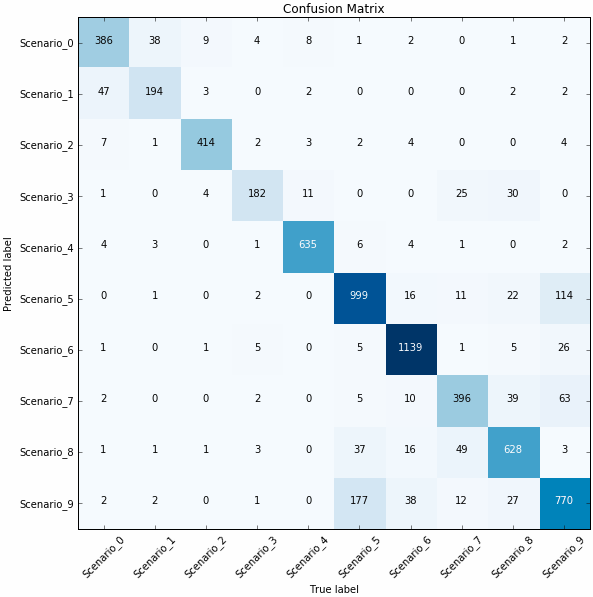
\includegraphics[width=\linewidth]{figures/knn_scaled_S_50}
        \caption{KNN-50 neighbors, StandardScaled, trained with small (S) dataset}
        \label{fig:knn_2}
    \end{subfigure}
    \begin{subfigure}[htb]{0.49\textwidth}
        \centering
        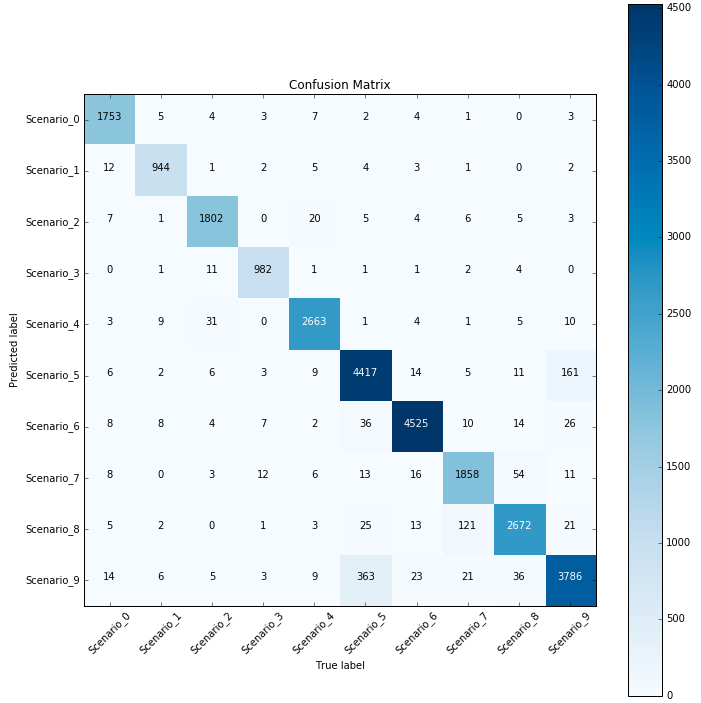
\includegraphics[width=\linewidth]{figures/knn_unscaled_XL_4}
        \caption{KNN-4 neighbors, unscaled, trained with whole (XL) dataset}
        \label{fig:knn_4}
    \end{subfigure}
    \caption{Confusion Matrixes for K-nearest Neighbor Models}
    \label{fig:confusionknn}
\end{figure}

\begin{figure}[!htb]
    \captionsetup[subfigure]{justification=centering}
    \centering
    \begin{subfigure}[htb]{0.49\textwidth}
        \centering
        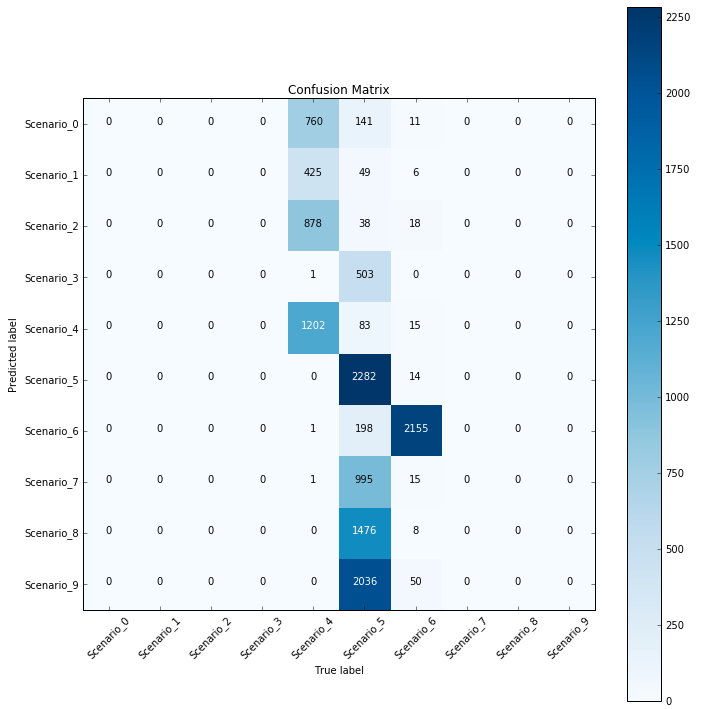
\includegraphics[width=\linewidth]{figures/dtc_unscaled_L_2}
        \caption{Decision Tree, unscaled, depth=2, trained with large (L) dataset}
        \label{fig:knn_2}
    \end{subfigure}
    \begin{subfigure}[htb]{0.49\textwidth}
        \centering
        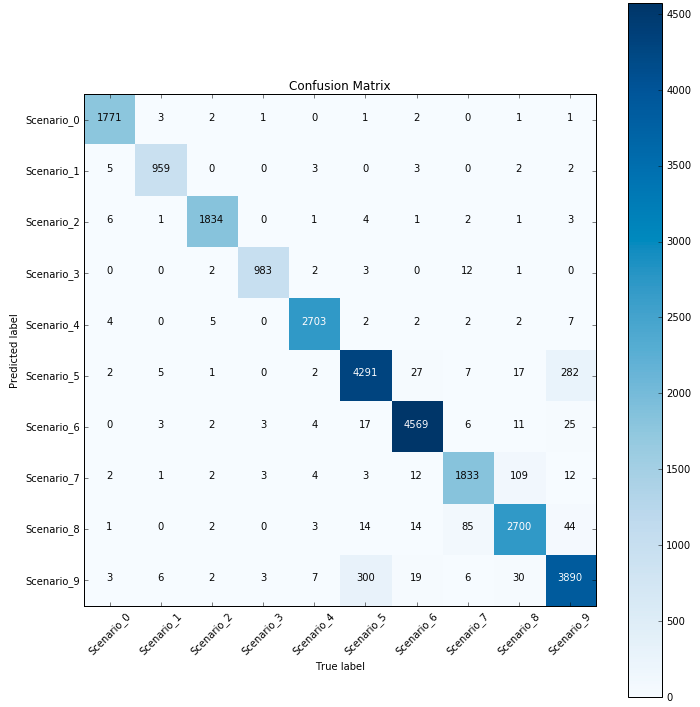
\includegraphics[width=\linewidth]{figures/dtc_unscaled_XL_50}
        \caption{Decision Tree, unscaled, depth=50, trained with whole (XL) dataset}
        \label{fig:knn_4}
    \end{subfigure}
    \caption{Confusion Matrixes for Decision Tree Models}
    \label{fig:confusiondtc}
\end{figure}
\begin{figure}[!htb]
    \captionsetup[subfigure]{justification=centering}
    \centering
    \begin{subfigure}[htb]{0.49\textwidth}
        \centering
        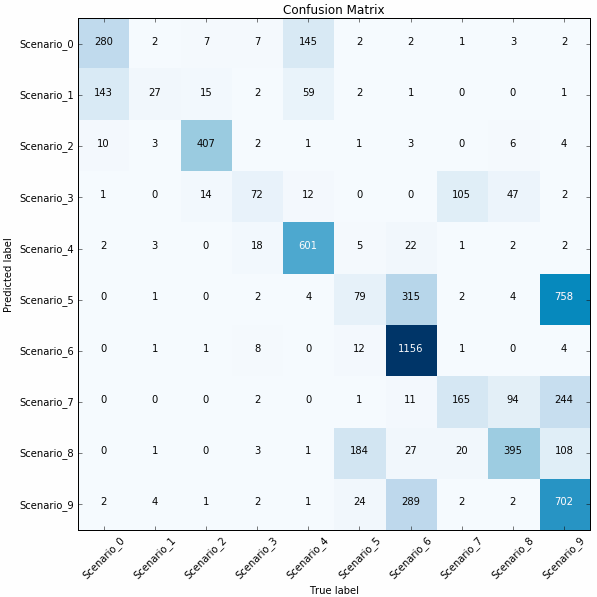
\includegraphics[width=\linewidth]{figures/svc_scaled_S_1}
        \caption{\ac{SVM}, StandardScaled, \(\gamma=2^{-9}\), trained with small (S) dataset}
        \label{fig:knn_2}
    \end{subfigure}
    \begin{subfigure}[htb]{0.49\textwidth}
        \centering
        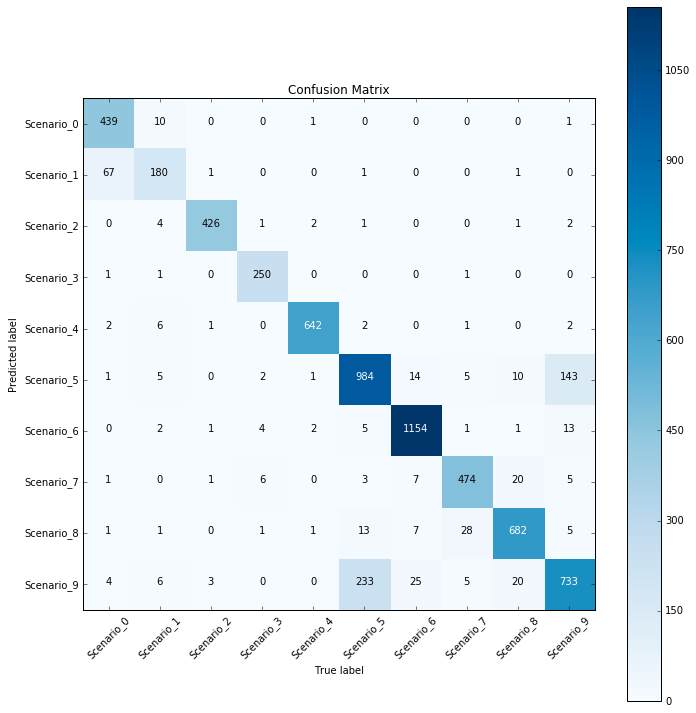
\includegraphics[width=\linewidth]{figures/svc_scaled_S_1e6}
        \caption{\ac{SVM}, StandardScaled, \(\gamma=2^3\), trained with small (S) dataset}
        \label{fig:knn_4}
    \end{subfigure}
    \caption{Confusion Matrixes for \ac{SVM} Models}
    \label{fig:confusionsvc}
\end{figure}
It is also important to notice the clear difference on the number of samples present for each scenario. This is due to the fact that the measurements performed in section~\ref{ch:measure} were based on runtime and not on number of generated samples, and the feature extraction algorithm described in section~\ref{ch:features} generates a different number of samples for each scenario, because of its dependence on the \emph{frame events} generation consequently of the channel occupation and interframe time of arrival itself. A different approach for feature extraction based on a number of features generated is proposed in chapter~\ref{ch:conclusions}.

From these matrices it can be clearly seen, at a first glance, that the K-Nearest algorithm and the decision trees perform quite well regardless of its configuration, having a more populated diagonal in its confusion matrix in comparison with the \ac{SVM} models. Additionally, just a small improvement in the classification accuracy is seen as the complexity and dataset size increases for this model. In general, it is safe to assert that the classification performs generally well for most of the scenarios except scenario 5, where a higher number of false positives, as well as false negatives, is seen for all models, being misclassified as scenario 9. This indicates that the extracted features for these specific scenarios have a noticeable correlation, which is not utterly surprising given that these scenarios share the channel occupation and interframe delay, being different only in the distribution with which the interframe delay is set: deterministic for scenario 5 and stochastic, with Poisson distribution, for scenario 9. This serves as an invitation to determine a feature that confidently sets a difference between them.
\subsection{Image Classification}\label{ch:image_classification}
For the image classification part of this work, a sequential model based on the work of \cite{Paisana2017} was implemented. The basic structure of this model is shown in Fig~\ref{fig:cnn}. As it can be seen, the model is composed of the connection of different layers, each of them with an specific functionality:

\begin{figure}[!htb]
    \centering
      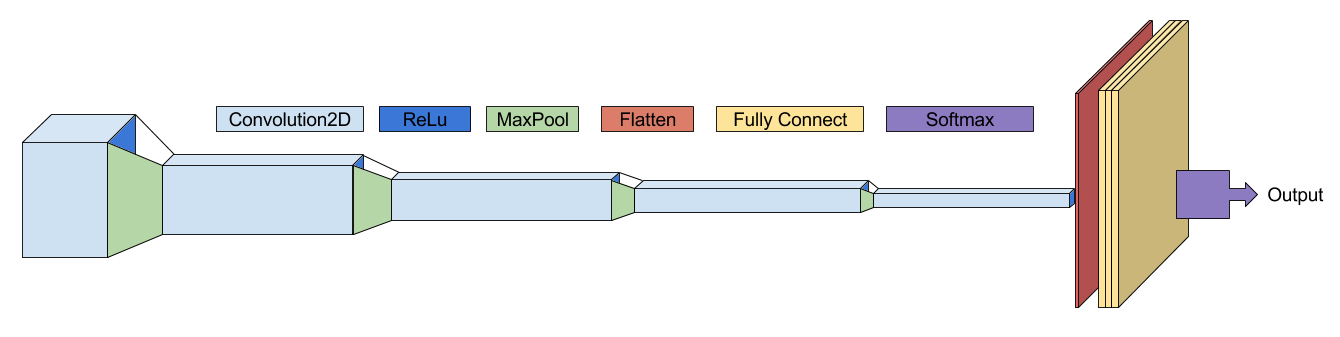
\includegraphics[width=\textwidth]{figures/cnn}
      \caption{Schema of the implemented CNN}
      \label{fig:cnn}
\end{figure}

\begin{itemize}
    \item Convolution2D: this comprises a convolutional kernel. It convolves the input to produce tensors at its output. This is the backbone of the \ac{ConvNet}, as it is the responsible for learning. Here, 2-Dimensional convolutional blocks of kernel size 2x2 are applied, as it is convolving over the area of the input images.
    \item MaxPool: this layer serves its purpose for dimension reduction, which is a form of downsampling. Briefly, it divides the input tensor into 2x2 non-overlapping squares and keeps the largest value present in each of these cells, effectively reducing the size of the representation, which in consequence reduces the number of parameters transitting the network. This has the effect of reducing the number of vector operations as well, making each layer of the network less processing-demandant. Additionally, as parameters are being dropped, this helps to avoid overfitting by disregarding eventual characteristics that are being "memorized". The principle of operation of such layers is shown in Fig~\ref{fig:maxpool}.
        \begin{figure}[!htb]
            \centering
              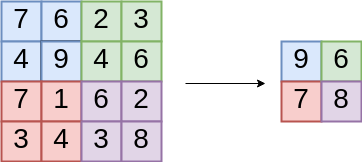
\includegraphics[width=0.4\textwidth]{figures/maxpool}
              \caption{2-D MaxPool}
              \label{fig:maxpool}
        \end{figure}
    \item \ac{ReLu}: this is an activation layer, i.e. a layer that applies a function that defines the type of output depending on its input. In the \ac{ReLu} case, the applied function is \(f(x) =\max(0,x) \), where x is the input of the neuron. Being a non-linear function, this activation increases the nonlinearity of the network without affecting the visual field, as there is no reduction of dimension.
        \begin{figure}[!htb]
            \centering
                \begin{tikzpicture}[scale=0.9]
                    \begin{axis}[
                        xlabel={$x$},
                        ylabel={$f(x)$},
                    ]
                        \addplot[domain=0.001:3,samples=201,purple,thick,smooth]{x};
                        \addplot[domain=-3:0.001,samples=201,purple,thick,smooth]{0};
                    \end{axis}
                \end{tikzpicture}
              \caption{ReLu activation function}
              \label{fig:maxpool}
        \end{figure}
    \item Fully connected layer: as the name states, this layer is connected to each one of the activations of the previous layers. These type of layers are the principle of operation of traditional neural networks, and is in charge of learning the non-linearities that have been propagated throughout the network.
    \item Softmax: this is also an activation layer. It takes vector q of dimension K and compress it together with values that add up to one. The function is given by
        \begin{equation}
            P(q)_i = \frac{e^{q_i}}{\sum_{k=1}^{K} \exp{q_j}}
        \end{equation}

        It can be easily understood that the dimension of the output from this softmax function is the number of labels to classify and that the value of each is the probability of the input sample to belong to that class. Consequently, the classification result is the \( \argmax \) of the function output.
\end{itemize}

The chosen layers and its disposition are strictly related to the input. In this case, the input picture has a 64x64 size, which describes then the height and width of the first layer. The depth is the number of filters that are used for each layer, and it is, to some extent, represented in the extension of the scale of Fig~\ref{fig:cnn}. 5 convolutional layers, with kernel dimensions 2x2, were used in this sequential model, with depths of 48, 128, 192, 192 and 128 filters correspondingly. At the end of the sequential model, 3 fully connected layers with depth 1024, 1024 and 10 were used. The succession of dimension changes of the sequential model and the number of parameters considered in each of the stages of the classification problem is summarized in Table~\ref{table:convnet_summary}. The number of parameters is the number of trainable weights that each layer contains. For a convolutional layer, this is calculated as \( \text{\# parameters} = \text{(depth of input tensor)}\cdot\text{(depth output tensor)}\cdot\text{height}_{kernel}\cdot \text{width}_{kernel} + \text{(depth output tensor)} \). As an example, the calculation for the first layer gives:
\begin{equation*}
    1 \cdot 48 \cdot 2 \cdot 2 + 48 = 240
\end{equation*}

\begin{table}[h!]
    \centering
    \begin{tabular}{|c|c|c|}
        \hline
        \textbf{Layer} & \textbf{Output Shape} & \textbf{\# Parameters} \\
        \hline\hline
        Convolution \# 1 & (63, 63, 48) & 240 \\\hline
        ReLu \# 1 & (63, 63, 48) & 0 \\\hline
        MaxPooling \# 1 & (31, 31, 48) & 0 \\\hline
        Convolution \# 2 & (30, 30, 128) & 24704 \\\hline
        ReLu \# 2 & (30, 30, 128) & 0 \\\hline
        MaxPooling \# 2 & (15, 15, 128) & 0 \\\hline
        Convolution \# 3 & (14, 14, 192) & 98496 \\\hline
        ReLu \# 3 & (14, 14, 192) & 0 \\\hline
        MaxPooling \# 3 & (7, 7, 192) & 0 \\\hline
        Convolution \# 4 & (6, 6, 192) & 147648 \\\hline
        ReLu \# 4 & (6,6, 192) & 0 \\\hline
        MaxPooling \# 4 & (3, 3, 192) & 0 \\\hline
        Convolution \# 5 & (2, 2, 128) & 98432 \\\hline
        ReLu \# 5 & (2,2, 128) & 0 \\\hline
        MaxPooling \# 5 & (1, 1, 128) & 0 \\\hline
        flatten & 128 & 0 \\\hline
        Fully Connected \#1 & 1024 & 132096 \\\hline
        Fully Connected \#2 & 1024 & 1049600 \\\hline
        Fully Connected \#3 & 10 & 10250 \\\hline
        Softmax & 10 & 0 \\\hline
        \hline
    \end{tabular}
    \caption{ConvNet dimensions and Number of Parameters}
    \label{table:convnet_summary}
\end{table}

The sequential model performs an optimization over its error function, for which the optimizer used can be selected. Keras provides a variety of these optimizers, using the approach of the steepest descent optimization over an objective function, \(J(\theta)\) with \(\theta \in \mathbb{R}^{d}\), being \(d\) the dimension of the objective function, by updating the parameters in the opposite direction of the gradient of \(J\), i.e.

\begin{equation}
    \nabla_\theta J(\theta) \text{  w.r.t } \theta, x, y
\end{equation}

A tunable parameter is the learning rate \(\eta\), that determines the size of the steps taken to reach the minimum. For this work, three different optimizers were used and analyzed based on the resulting accuracy of the classification over the test data, as well as its value for error during validation.

\begin{itemize}
    \item Stochastic gradient descent: this algorithm performs a parameter update after each training sample
        \begin{equation}
            \theta = \theta - \eta \cdot \nabla_\theta J(\theta;x^i;y^i)
        \end{equation}
        This optimizer was used in \cite{Paisana2017} and was used as a baseline. The learning rate \(\eta\) was decreased every one-fourth of the total iterations, which in this specific use case was set to 3000. Decreasing the learning rate increases the chance that this optimizer reaches a local minimum.
    \item Adadelta \cite{Zeiler2012a}: this optimizer is based on the Adagrad optimizer \cite{Duchi2011}, which adapts intrinsically its learning rate to the parameters, therefore doing bigger updates for infrequent parameters, and smaller updates for frequent ones. It is proven that this optimizer is more robust than the stochastic gradient descent \cite{Duchi2011} by storing all previous squared gradients and updating accordingly. Adadelta extends this robustness by restricting the amount of accumulated squared gradients to a fixed window, and using this accumulation for its updates.
    \item Adamax: based on the Adaptive Moment Estimation - Adam \cite{Kingma2014}, this optimizer also sets an adaptive learning rate based on the parameters of the objective function. Additionally, to set a fixed window of past squared decays as Adadelta, Adam also keeps an exponentially decaying average of past gradients, which is similar to a momentum \cite{Dahl2013}. Adamax extends Adam functionality by maximizing the norm of the update vector, which leads to a stable behavior.
\end{itemize}

The validation of the models was performed based on the accuracy that these optimizers have during training and testing, the loss factor during the same stages, which is a measure of the error provided by the optimization process. The results are shown in Figs~\ref{fig:sgd}, \ref{fig:adamax} and \ref{fig:adadelta}.

\begin{figure}[!htb]
    \centering
    \begin{subfigure}[htb]{0.49\textwidth}
        \centering
        \begin{tikzpicture}[scale=0.8]
            \begin{axis}[
                xlabel={Iterations},
                ylabel={Loss Factor},
                  ]
                \addplot table [x=epoch, y=loss, col sep=comma, mark=none] {data/sgd.csv};
                \addplot table [x=epoch, y=val_loss, col sep=comma, mark=none] {data/sgd.csv};
                \legend{Training loss, Validation loss}
        \end{axis}
        \end{tikzpicture}
    \end{subfigure}
        \hfill
    \begin{subfigure}[htb]{0.49\textwidth}
        \centering
        \begin{tikzpicture}[scale=0.8]
            \begin{axis}[legend pos=south east,
                xlabel={Iterations},
                ylabel={Accuracy},
                  ]
                \addplot table [x=epoch, y=acc, col sep=comma, mark=none] {data/sgd.csv};
                \addplot table [x=epoch, y=val_acc, col sep=comma, mark=none] {data/sgd.csv};
                \legend{Accuracy, Validation Accuracy}
        \end{axis}
        \end{tikzpicture}
    \end{subfigure}
    \caption{Metrics for Steepest Gradient descent Optimizer}
    \label{fig:sgd}
\end{figure}


\begin{figure}[!htb]
    \centering
    \begin{subfigure}[htb]{0.49\textwidth}
        \centering
        \begin{tikzpicture}[scale=0.8]
            \begin{axis}[
                xlabel={Iterations},
                ylabel={Loss Factor},
                  ]
                \addplot table [x=epoch, y=loss, col sep=comma, mark=none] {data/adamax.csv};
                \addplot table [x=epoch, y=val_loss, col sep=comma, mark=none] {data/adamax.csv};
                \legend{Training loss, Validation loss}
        \end{axis}
        \end{tikzpicture}
    \end{subfigure}
        \hfill
    \begin{subfigure}[htb]{0.49\textwidth}
        \centering
        \begin{tikzpicture}[scale=0.8]
            \begin{axis}[legend pos=south east,
                xlabel={Iterations},
                ylabel={Accuracy},
                  ]
                \addplot table [x=epoch, y=acc, col sep=comma, mark=none] {data/adamax.csv};
                \addplot table [x=epoch, y=val_acc, col sep=comma, mark=none] {data/adamax.csv};
                \legend{Accuracy, Validation Accuracy}
        \end{axis}
        \end{tikzpicture}
    \end{subfigure}
    \caption{Metrics for Adamax Optimizer}
    \label{fig:adamax}
\end{figure}

\begin{figure}[!htb]
    \centering
    \begin{subfigure}[htb]{0.49\textwidth}
        \centering
        \begin{tikzpicture}[scale=0.9]
            \begin{axis}[
                xlabel={Iterations},
                ylabel={Loss Factor},
                  ]
                \addplot table [x=epoch, y=loss, col sep=comma, mark=none] {data/adadelta.csv};
                \addplot table [x=epoch, y=val_loss, col sep=comma, mark=none] {data/adadelta.csv};
                \legend{Training loss, Validation loss}
        \end{axis}
        \end{tikzpicture}
    \end{subfigure}
    \hfill
    \begin{subfigure}[htb]{0.49\textwidth}
        \centering
        \begin{tikzpicture}[scale=0.9]
            \begin{axis}[legend pos=south east,
                xlabel={Iterations},
                ylabel={Accuracy},
                  ]
                \addplot table [x=epoch, y=acc, col sep=comma, mark=none] {data/adadelta.csv};
                \addplot table [x=epoch, y=val_acc, col sep=comma, mark=none] {data/adadelta.csv};
                \legend{Accuracy, Validation Accuracy}
        \end{axis}
        \end{tikzpicture}
    %}
    \end{subfigure}
    \caption{Metrics for Adadelta Optimizer}
    \label{fig:adadelta}
\end{figure}

From these plots, it can clearly be seen that SGD takes a greater number of iterations to reach its maximum accuracy as well as its minimum loss factor in comparison with Adamax and Adadelta. With respect to their comparative accuracies, it is not conclusive that one of the optimizers provide a better result. The maximum and final values of the accuracies of these models are shown in Table~\ref{table:convnet_accs}, whilst the minimum and final values for the loss factor is shown in Table~\ref{table:convnet_loss}.

\begin{table}[!ht]
  \centering
    \begin{tabular}{| >{\centering\arraybackslash}m{5em}| >{\centering\arraybackslash}m{7em}| >{\centering\arraybackslash}m{7em}| >{\centering\arraybackslash}m{7em}| >{\centering\arraybackslash}m{7em}|}
    \cline{2-5}
      \multicolumn{1}{c|}{} & Max Training Accuracy (Iter) & Final Training Accuracy & Max Validation Accuracy (iter) & Final Validation accuracy \\ \hline
      SGD & 99\% (2411)   & 98\%   & 90\% (981) & 81\%  \\ \hline
      Adamax & 92\% (2997)   & 88\%   & 87\% (2679) & 77\%  \\ \hline
      Adadelta & 100\%(2012)   & 99.6\%   & 89\% (489) & 85\%  \\ \hline
  \end{tabular}
    \caption{Maximum and Final Accuracies for ConvNets with various optimizers}
    \label{table:convnet_accs}
\end{table}


\begin{table}[!ht]
  \centering
    \begin{tabular}{| >{\centering\arraybackslash}m{5em}| >{\centering\arraybackslash}m{7em}| >{\centering\arraybackslash}m{7em}| >{\centering\arraybackslash}m{7em}| >{\centering\arraybackslash}m{7em}|}
    \cline{2-5}
      \multicolumn{1}{c|}{} & Min Training Loss (Iter) & Final Training Loss & Min Validation Loss (iter) & Final Validation Loss \\ \hline
  SGD & 0.625 (2866)   & 0.64   & 0.863 (861) & 1.134  \\ \hline
      Adamax & 0.24 (2997)   & 0.37   & 0.47 (1150) & 0.93  \\ \hline
      Adadelta & 0.03 (2998)   & 0.04   & 0.4 (297) & 0.74  \\ \hline
  \end{tabular}
    \caption{Maximum and Final Loss Factor for ConvNets with various optimizers}
    \label{table:convnet_loss}
\end{table}

The low values for losses as well as high values for accuracies in the training process do not come as a surprise, but it is the iteration where they are reached what is significant to be analyzed, as they state the rate of convergence of each of the optimizers. For the training phase, it is also expected that these values are constantly increasing along the whole process, as the model keeps learning from the data and fits to it. Therefore, it is of special interest to focus the attention to the validation part. Regarding the accuracy value, it is not conclusive to determine an algorithm that outperforms the others. Additionally, an accuracy greater than 87\% for all the optimizers is satisfactory, keeping in mind that these models are trained with spectrograms with SNR as low as -5dB, where the \ac{PU} signal is well below the noise level. It is clear that the rate of convergence of Adadelta surpasses the performance of the other optimizers, for both the maximum validation accuracy and the minimum validation loss, which states that using early stop techniques allows having a satisfactory model with short training time. More insights about the early stop techniques are given in the following chapter, where it will be clear why the maximum validation accuracy and minimum validation loss are important values to be considered.

Looking carefully at the loss factor plots for validation, a clear tendency of the increase of this parameter at the end of the iterative process can be seen for the Adamax and Adadelta optimizers, which is an indication of overfitting. Although not clear from the plots, SGD also shows overfitting behavior to some extent, as it can be seen in the noticeable difference on the maximum accuracy vs the final accuracy in table~\ref{table:convnet_accs}.


  \acresetall
\chapter{Live implementation in GNURadio}\label{chapter:live} \label{ch:live}

%  \acresetall
% This is an example chapter from 'Polar Codes for Software Radio'. Do not use it but delete it! It serves as an example!
\chapter{System model}\label{chapter:systemmodel}
Polar codes are defined for a specific system model.
The objective of this chapter is to introduce the key concepts.
Notations are introduced and important terms are revisited in order to refer to them.

\section{Key channel coding concepts}
The system model used throughout this thesis follows the remarks in \cite{Richardson:2008:MCT} and \cite{polar:arikan09}.
It is intended to define the domain for which polar codes are developed.

The objective of channel coding is to transmit information from a source to a sink over a point-to-point connection with as few errors as possible.
A source wants to transmit binary data  $u \in \mathcal{U} = \{0, 1\}$ to a sink where $u$ represents one draw of a binary uniformly distributed random variable.
The source symbols are encoded, transmitted over a channel and decoded afterwards in order to pass an estimate $\hat{u}$ to a sink.

This thesis uses a common notation for vectors which is introduced here shortly.
A variable $x$ may assume any value in an alphabet $x \in \mathcal{X}$.
Multiple variables are combined into a vector $x^N = (x_0, \dots , x_{N-1})$ of size $N$ with its alphabet $x^N \in \mathcal{X}^N$.
A subvector of $x^N$ is denoted $x_i^j = (x_i, \dots, x_{j-1})$ where $0 \leq i \leq j \leq N$.
A vector where $i=j$ is an empty vector.
A vector $x^N$ may be split into even and odd subvectors which are denoted $x_{0,e}^{2n} = (x_0, x_2, \dots, x_{2n-2})$, $x_{0,o}^{2n} = (x_1, x_3, \dots, x_{2n-1})$.
This numbering convention is in accordance with \cite{dijkstra:zerocounting}, where the author makes a strong point for this exact notation and some papers on polar codes follow it too, e.g. \cite{polar:talvardy:howtoCC}.


\subsection{Encoder}
The encoder takes a frame $u^k$ and maps it to a binary codeword $x^N$, where $k$ and $N$ denote the vector sizes of a frame and a codeword respectively with $k \leq N$.
An ensemble of all valid codewords for an encoder is a code $\mathcal{C}$.
It should be noted that $|\mathcal{C}| = |\mathcal{X}^N|$ must hold in order for the code to be able to represent every possible frame.

Not all possible symbols from $\mathcal{X}^N$ are used for transmission.
The difference between all possible codewords $2^N$ and used codewords $2^k$ is called redundancy.
With those two values, the code rate is defined as $R = \frac{k}{N}$.
It is a measure of efficient channel usage.

The encoder is assumed to be linear and to perform a one-to-one mapping of frames to codewords.
A code is linear if $\alpha x + \alpha' x' \in \mathcal{C}$ for $\forall x, x' \in \mathcal{C}$ and $\forall \alpha, \alpha' \in \mathbb{F}$ hold.
It should be noted that all operations are done over the Galois field GF(2) or $\mathbb{F} = \{0, 1\}$ if not stated otherwise.
Then the expression can be simplified to 
\begin{equation}
 x + x' \in \mathcal{C} \quad \textrm{for} \quad \forall x, x' \in \mathcal{C}.
\end{equation}
A linear combination of two codewords must yield a codeword again.

For linear codes it is possible to find a generator matrix $G \in \mathbb{F}^{k \times N}$ and obtain a codeword from a frame with $x^N = u^k G^{k \times N}$.
All linear codes can be transformed into systematic form $G = I_k P$.
$I_k$ is a $k \times k$ dimensional identity matrix.
If $G$ is systematic, all elements of a frame $u^k$ are also elements of the codeword $x^N$.
Also, a parity check matrix $H = -P^T I_{N-k}$ with dimensions $(N-k) \times N$ can be calculated from $G$.
A parity check matrix satisfies $\forall x \in \mathcal{C}: H x^T = 0^T $.
Thus, a parity check matrix can be used to verify correct codeword reception and furthermore error correction may be performed.
Error correction with $H$ may be done, e.g. syndrome decoding.

A code can be characterized by the minimum distance between any two codewords.
In order to obtain this value we use the Hamming distance.
This distance $d(v^N,x^N)$ equals the number of positions in $v^N$ that differ from $x^N$.
Minimum distance of a code is than defined by $d(\mathcal{C}) = \min\{d(x,v): x,v \in \mathcal{C}, x \neq v\}$.
For linear codes this can be simplified to comparing all codewords to the zero codeword $d(\mathcal{C}) = \min\{d(x,0): x \in \mathcal{C}, x \neq 0\}$ which is called Hamming weight.

\subsection{Channel model}\label{sec:channel_model}
Channel coding relies on a generic channel model.
Its input is $x \in \mathcal{X}$ and its distorted output is $y \in \mathcal{Y}$.
A channel is denoted $W: \mathcal{X} \rightarrow \mathcal{Y}$ along with its transition probability $W(y|x), x \in \mathcal{X}, y \in \mathcal{Y}$.
A \ac{DMC} does not have memory, thus every symbol transmission is independent from any other.
Combined with a binary input alphabet it is called a \ac{BDMC}.
For a symmetric channel model, $P(y|1) = P(-y|-1)$ must hold for an output alphabet $y \in \mathcal{Y}, \mathcal{Y} \subset \mathbb{R}$ \cite{Richardson:2008:MCT}.
Assuming symmetry for a \ac{BDMC} leads to a symmetric \ac{BDMC}.
In Sec. \ref{theory:channels} several examples of such channels are discussed.

This channel concept may be extended to vector channels.
A vector channel $W^N$ corresponds to $N$ independent uses of a channel $W$ which is denoted as $W^N : \mathcal{X}^N \rightarrow \mathcal{Y}^N$.
Also, vector transition probabilities are denoted $W^N(y^N|x^N) = \prod_{i=0}^{N-1} W(y_i|x_i)$.

\subsection{Decoder}
A decoder receives a possibly erroneous codeword $y$ and checks its validity by asserting $H y^T = 0^T$, thus performing error detection.
A more sophisticated decoder tries to correct errors by using redundant information transmitted in a codeword.
An optimal decoder strategy is to maximize the a-posteriori probability.
Given the probability of each codeword $P(x)$ and the channel transition probability $P(y|x)$, the task at hand is to find the most likely transmitted codeword $x$ under the observation $y$, $P(x|y)$.
This is denoted
\begin{equation}
 \hat{x}^{MAP} = \argmax_{x \in \mathcal{C}} p(x|y) = \argmax_{x \in \mathcal{C}} p(y|x) \frac{p(x)}{p(y)} = \argmax_{x \in \mathcal{C}} p(y|x) p(x)
\end{equation}
with Bayes' rule.
Assume every codeword is transmitted with same probability $P(x^{(i)}) = P(x^{(j)}), \; \forall x^{(i)}, x^{(j)} \in \mathcal{C}$.
This simplifies the equation and yields a \ac{ML} decoder
\begin{equation}
 \hat{x} = \argmax_{x \in \mathcal{C}} p(y|x)
\end{equation}
which estimates the most likely codeword to be transmitted given a received possibly erroneous codeword \cite{Richardson:2008:MCT}.
This decoding principle could be employed in conjunction with the Hamming distance and thus yield $\hat{x} = \argmin_{x \in \mathcal{C}} d(x, y)$.
In conclusion the task at hand is to find a code which inserts redundancy intelligently, so a decoder can use this information to detect and correct transmission errors.

\subsection{Asymptotically good codes}\label{theory:repetition_code}
A repetition code is a very simple code which helps clarify certain key concepts in the channel coding domain.
Assume the encoder and decoder use a repetition code.
For example a repetition code with $k=1$ and $N = 3$ has two codewords $\mathcal{C} = \{000, 111\}$.
Thus in this example $R=\frac{1}{3}$.
We can also obtain its generator and parity check matrices.
\begin{equation}
 G = \begin{pmatrix} 1 & 1 & 1 \end{pmatrix},\qquad H = \begin{pmatrix} 1 & 1 & 0 \\ 1 & 0 & 1 \end{pmatrix}
\end{equation}
$H$ can be used to detect if a transmission error occurred by verifying if $H x^T = 0^T$.
In case an error occurred, a \ac{ML} decoder does a majority decision to estimate the most likely codeword.

Repetition codes shed light on a problem common to a lot of codes.
If reliability of a code needs to be improved, it comes at the expense of a lower code rate.
Increasing $N$ comes at the expense of decreasing $R = \frac{1}{N}$ because $k=1$ for all repetition codes.
Thus for a very reliable repetition code $\lim_{N \rightarrow \infty} R$ tends towards $0$.

The above results leads to the definition of asymptotically good codes $\mathcal{C}(N_s, k_s, d_s)$ \cite{Friedrichs:2010:error-control-coding}.
Two properties must hold for this class of codes,
\begin{equation}
 R = \lim_{s \rightarrow \infty} \frac{k_s}{N_s} > 0 \quad \textrm{and} \quad  \lim_{s \rightarrow \infty} \frac{d_s}{N_s} > 0.
\end{equation}
The code rate must be $>0$ for all codes which repetition codes do not satisfy.
And the distance between codewords must grow proportionally to the code block size.

\section{Channels}\label{theory:channels}
Several common channel models exist to describe the characteristics of a physical transmission.
Common properties were discussed in Section \ref{sec:channel_model} whereas in this Section the differences are targeted.
The three most important channel models for polar codes are presented, namely the \ac{BSC}, the \ac{BEC} and the \ac{AWGN} channel.

\subsection{AWGN channel}
An \ac{AWGN} channel as used in this thesis has a binary input alphabet and a continuous output alphabet $\mathcal{Y} = \mathbb{R}$.
Each input symbol is affected by Gaussian noise to derive an output symbol.
Its average corresponds to the input symbol value and the variance can be interpreted as a measure of noise.
Often the input is \ac{NRZ} encoded which turns a \ac{ML} decision for a symbol into a sign decision.

\subsection{Capacity and reliability}
Channels are often characterized by two important measures, capacity and reliability.
These measures are introduced in this Section.
Channel capacity for symmetric \ac{BDMC} can be calculated by
\begin{equation}
 I(W) = \frac{1}{2} \sum_{y \in \mathcal{Y}} \sum_{x \in \mathcal{X}} W(y|x) \log_2 \frac{W(y|x)}{\frac{1}{2} (W(y|0) + W(y|1))}.
\end{equation}
It defines the highest rate at which a reliable transmission over a channel $W$ can be conducted while the error probability may still tend towards $0$.
It is also called the Shannon capacity \cite{sha49} for symmetric channels.
The Bhattacharyya parameter
\begin{equation}
 Z(W) = \sum_{y \in \mathcal{Y}} \sqrt{W(y|0) W(y|1)}
\end{equation}
is used to quantify a channel's reliability where a lower value for $Z(W)$ indicates higher reliability.
It is also referred to as Z-parameter for obvious reasons.
Also, an upper \ac{ML} decision error bound is given by $Z(W)$ \cite{polar:arikan09}.
		% an example chapter
  \chapter{Conclusion}\label{chapter:conclusion} \label{ch:conclusions}
Using the setup of the DySpan Spectrum Challenge 2017, the identified need was to determine the transmission fashion that the \ac{PU} has, which switched randomly between ten different scenarios, each one with different characteristics. Although it represents a complex exercise to try to describe this behavior analyticallly, it was observed that each scenario had a clear pattern, and that this pattern could be recorded for further analysis, making this a suitable situation in which machine learning techniques could be applied, and it is shown in this work that these methods provide a satisfactory performance on providing spectrum awareness for interweave systems.

Two main learning techniques are proposed:

\begin{itemize}
    \item feature-based learning using K-nearest neighbors, decision trees and support vector machines classifiers
    \item spectrogram-based learning using convolutional neural networks and different optimizers such as stochastic gradient descent, adamax and adadelta.
\end{itemize}

The feature-based classifiers have a satisfactory performance, reaching up to 95\% of accuracy and representing an improvement over the implementation used in the DySpan Spectrum Challenge in the way that a comparable accuracy is obtained for high SNR values without having to describe the PU procedure analytically . However, they have the inherent limitation from the energy detection based feature extraction, which only allows these classifiers to make decisions in the presence of relatively high (>5dB) PU SNR. Additionally, it is seen that there is still a high correlation between the features for scenario 5 and scenario 9 (scenarios with full bandwidth occupation and same average interframe delay, varying solely in their interframe delay distribution: deterministic for the former, Poisson for the latter). This leads to misclassification even on situations where the \ac{PU} \ac{SNR} is high. This is an invitation to invest further effort on identifying a feature that separates these two scenarios with a higher confidence. Apart from this drawback, for situations where the \ac{PU} power is relatively high, very simple classifiers can be implemented with very small datasets and surprisingly low training and prediction times. K-nearest neighbors and decision trees are recommended for such situations, providing an accuracy up to 98\% with solely the equivalent of 2.5 minutes of recorded data, being able to generate a prediction in less than 200ms and 2ms respectively. Support vector machines, in the configuration that was analyzed in this work, are noticeable worse performing, taking several times longer to train and to predict. Furthermore, they are sensitive to scaling, which represents an additional step in data preprocessing, and therefore are less recommended for this specific use-case.


Spectrograms classifiers require a longer time to train than the feature-based classifiers. Nevertheless, using techniques as the model checkpoint, reliable models such as the Sequential model using Adadelta optimizer could be generated with a training as short as 297 iterations. In the consumer, off-the-shelf, laptop on which this model was trained, this represents a training as short as 30 minutes, being outstandingly accessible for fast implementations  providing superior results. For deep learning approaches, this sequential model with an Adadelta optimizer is recommended.
Furthermore, the need for dedicated hardware for image classification is gradually decreasing with the expanding number of cloud services for this type of procedures. Being able to use dedicated remote hardware could lead to a fast generation of convolutional networks which could potentiate experimentation and research.

As product of this work a reproducible testbed is generated, which serves as a kick-off point for fast experimentation using learning techniques in real communications systems. There are several other machine learning algorithms that are yet to be implemented, analyzed and benchmarked, for which this work serves as a reliable comparison framework. Moreover, although the recording of raw I/Q samples for this work required up to 300GB of hard disk space, the number of samples after preprocessing (around 80.000 features/label pairs and around 85.000 images for classification) are still considered a small dataset. With an improved file management, analysis of these training techniques with a bigger dataset is of special interest for future work. Besides, this work focused on keeping the configuration as loyal to the Spectrum Challenge as possible. However, a careful reduction of the sampling rate should not lead to any functionality difference, leading to less hard disk space needs and, consequently, allowing longer observations.

Also, the approach for the \ac{PU} measurements was based on fixed recording times which for the feature generation process leads to a different amount of samples depending on the scenario. Different approaches to achieve bigger datasets, such as counting generated features at the recording system might be worth further investigation.

Lastly, although satisfactory results are achieved on spectrum awareness, being able to confidently identify the way the \ac{PU} is accessing to the spectrum, it is paramount to extend the functionality of this awareness to the situation in which the \ac{SU} is able to effectively use the time and frequency slots available without interfering the ongoing communication link. Enhancing the results captured in this work to an adaption mechanism in which effective access to the spectrum is granted to the \ac{SU} transmitter would be a valuable step forward in the real implementation of interweave systems.
		% everything ends with a summary!


%% Appendix
\appendix
%  \listoffigures		% if you want, not usual
%  \listoftables		% if you want, not usual
  % This file provides Abbreviations
% Sorting them is a good idea because the acronym package won't!
\chapter{Abbreviations}
\begin{acronym}[TROLL]
  \acro{AGC}[AGC]{Automatic Gain Control}
  \acro{AKF}[AKF]{Autokorrelationsfunktion}
  \acro{AI}[AI]{Artificial Intelligence}
  \acro{API}[API]{Application Program Interface}
  \acro{AWGN}[AWGN]{Additive White Gaussian Noise}
  \acro{AVX}[AVX]{Advanced Vector Extensions}

  \acro{BEC}[BEC]{Binary Erasure Channel}
  \acro{BER}[BER]{Bit-Error-Rate}
  \acro{BDMC}[BDMC]{binary \acs{DMC}}
  \acro{BP}[BP]{Belief Propagation}
  \acro{BSC}[BSC]{Binary Symmetric Channel}
  \acro{BW}[BW]{Bandwidth}

  \acro{CEL}[CEL]{Communications Engineering Lab}
  \acro{CGRAN}[CGRAN]{The Comprehensive GNURadio Archive Network}
  \acro{ComSoc}[ComSoc]{IEEE Communications Society}
  \acro{ConvNet}[ConvNet]{Convolutional Neural Networks}
  \acro{CPU}[CPU]{Central Processing Unit}
  \acro{CR}[CR]{Cognitive Radio}

  \acro{DFT}[DFT]{Discrete Fourier Transform}
  \acro{DL}[DL]{Deep Learning}
  \acro{DMC}[DMC]{Discrete Memoryless Channel}
  \acro{dSNR}[dSNR]{design-\ac{SNR}}
  \acro{DSP}[DSP]{Digital Signal Processing}
  \acro{DySpan}[DySpan]{Dynamic Spectrum Access Networks}

  \acro{ESA}[ESA]{European Space Agency}
  \acro{EMC}[EMC]{IEEE Electromagnetic Compatibility Society}

  \acro{FER}[FER]{Frame Error Rate}
  \acro{FFT}[FFT]{Fast Fourier Transform}
  \acro{FCC}[FCC]{Federal Coomunications Commision (USA)}

  \acro{GPP}[GPP]{General Purpose Processor}
  \acro{GRC}[GRC]{GNU Radio Companion}
  \acro{GUI}[GUI]{Graphical User Interface}

  \acro{NASA}[NASA]{National Aeronautics and Space Administration}
  \acro{LDPC}[LDPC]{Low-Density Parity-Check}
  \acro{SIMD}[SIMD]{Single Instruction Multiple Data}
  \acro{VOLK}[VOLK]{Vector-Optimized Library of Kernels}

  \acro{IDFT}[IDFT]{Inverse Discrete Fourier Transform}
  \acro{ITU}[ITU]{International Telecommunications Union}
  \acro{IEEE}[IEEE]{Institute of Electrical and Electronics Engineers}

  \acro{KIT}[KIT]{Karlsruhe Institute of Technology}

  \acro{LR}[LR]{Likelihood Ratio}
  \acro{LLR}[LLR]{Log Likelihood Ratio}
  \acro{LTE}[LTE]{Long Term Evolution}

  \acro{MAP}[MAP]{Maximum A-Posteriori}
  \acro{ML}[ML]{Machine Learning}

  \acro{NRZ}[NRZ]{Non-Return-to-Zero}

  \acro{Ofcom}[OFCOM]{U.K. Offices of Communications}
  \acro{OFDM}[OFDM]{Orthogonal frequency division multiplexing}
  \acro{OOT}[OOT]{out of tree}

  \acro{PDU}[PDU]{Protocol data unit}
  \acro{pip}[pip]{Pip Installs Packages}
  \acro{PSK}[PSK]{Phase Shift Keying}
  \acro{PU}[PU]{Primary User}
  \acro{PyBOMBS}[PyBOMBS]{Python Build Overlay Managed Bundled System}

  \acro{RBF}[RBF]{Radial Basis Function}
  \acro{RV}[RV]{Random Variable}
  \acro{RF}[RF]{Radio Frequency}

  \acro{SC}[SC]{Successive Cancellation}
  \acro{SCC}[SCC41]{Standards Coordinating Committee 41}
  \acro{SCL}[SCL]{Successive Cancellation List}
  \acro{SDR}[SDR]{Software-Defined Radio}
  \acro{SNR}[SNR]{Signal-to-Noise-Ratio}
  \acro{SPC}[SPC]{Single-Parity-Check}
  \acro{SSE}[SSE]{Streaming SIMD Extensions}
  \acro{SU}[SU]{Secundary User}
  \acro{SVM}[SVM]{Support Vector Machines}
  \acro{SWIG}[SWIG]{Simplified Wrapper and Interface Generator}

 \acro{UHD}[UHD]{\ac{USRP} Hardware Driver\texttrademark}
 \acro{UML}[UML]{Unified Modeling Language}
 \acro{USRP}[USRP]{Universal Software Radio Pheripheral}
\end{acronym}
	% use the acronym package. Already include with the template.
  \bibliography{lib}	% include bibliography.bib and with formating etc.


\end{document}
